\documentclass{article}
\usepackage{graphicx} % Required for inserting images
\usepackage[T1]{fontenc} 
\usepackage[francais]{babel}
\usepackage{lmodern}
\usepackage{listings}
\usepackage{xcolor}
\usepackage[ruled, french]{algorithm2e}
\usepackage{amsmath}
\usepackage{hyperref} % Pour les liens
\usepackage{subcaption} % Pour les sous figures
\usepackage{float}
\usepackage[bottom]{footmisc}
\usepackage{wrapfig}
\usepackage{algpseudocode}
\usepackage{tikz}
\definecolor{jsonKey}{rgb}{0.75, 0.1, 0.1}
\definecolor{jsonString}{rgb}{0.1, 0.5, 0.1}
\usetikzlibrary{positioning, shapes, arrows}
\lstdefinelanguage{json}{
    basicstyle=\ttfamily,
    showstringspaces=false,
    breaklines=true,
    frame=single,
    backgroundcolor=\color{gray!10},
    morestring=[b]",
    stringstyle=\color{jsonString},
    literate=
     *{:}{{\color{black}:\ }}{1}
      {,}{{\color{black},\ }}{1}
      {\{}{{\color{black}{\{}}}{1}
      {\}}{{\color{black}{\}}}}{1}
}
\title{Analyse des trajectoires de joueurs de Dota2}
\author{Alexandre Faupoint, Romain Moalic, Thomas Doguet, Etienne BOSSU\\ 
Sous la direction de M. BONNET Gregory}
\date


\begin{document}
    %Page de garde: affche title, author, date ci dessus
    \maketitle
\begin{center}
    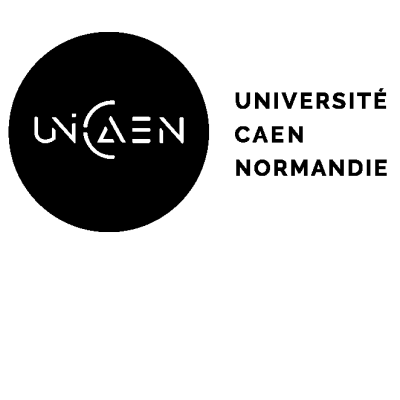
\includegraphics[width=10cm]{logoUnicaen.png}
    \end{center}

    %Pour que la page de garde ne compte pas dans la pagination:
    \thispagestyle{empty}
    \setcounter{page}{0}

    \newpage
    
    %Table des matières:
    \tableofcontents

    \newpage
    
    \section{Introduction}
   
        Dans le cadre de notre unité d'enseignement \textit{Projet 2}, nous avons mené une étude sur les stratégies adoptées par les joueurs de 	extit{Dota 2}, un jeu multijoueur en équipe et en temps réel, classé parmi les MOBA (Multiplayer Online Battle Arena). L'objectif principal de ce projet était de concevoir un programme en langage Python permettant d'extraire et d'analyser les trajectoires des joueurs afin d'identifier certaines stratégies mises en place par les équipes et les joueurs eux-mêmes.
    
        Pour ce faire, nous avons exploré plusieurs méthodes et algorithmes adaptés à ce type d'analyse. Tout d'abord, nous avons utilisé l'approche MDL (Minimum Description Length) pour compresser les trajectoires en séquences de segments représentatifs. Ensuite, nous avons appliqué une méthode de clusterisation afin de regrouper les segments similaires ; pour cela, nous avons choisi l'algorithme K-Means de façon arbitraire. Enfin, nous avons utilisé la bibliothèque \textit{prefixspan} pour extraire des motifs récurrents au sein des trajectoires des joueurs, permettant ainsi de mettre en évidence des schémas de déplacement et des tendances stratégiques.
    
        Toutefois, plusieurs défis ont émergé au cours du projet. Nous avons dû concevoir des structures de données adaptées pour représenter efficacement les trajectoires et assurer une gestion optimale des données massives. Un prétraitement a également été nécessaire pour nettoyer les données et éliminer les valeurs aberrantes. De plus, le choix et l'implémentation d'algorithmes efficaces ont constitué un enjeu majeur afin d'assurer une analyse pertinente et un affichage exploitable des résultats.
    
        Ce rapport détaille notre approche et nos choix méthodologiques. Nous commencerons par exposer nos objectifs concrets, puis nous décrirons les fonctionnalités que nous avons implémentées ainsi que leur fonctionnement technique. Ensuite, nous expliquerons comment ces différentes composantes s'articulent pour former un programme cohérent, avant de présenter les expérimentations réalisées et les résultats obtenus.
    
    

    \section{Objectifs}

        \textit{Dota 2} est un jeu en équipe multijoueur en temps réel, opposant deux équipes de cinq joueurs sur une carte composée de trois routes principales : la route du haut (top), la route du milieu (mid) et la route du bas (bot), ainsi que d'une jungle qui les entoure. Chaque joueur endosse un rôle spécifique et contribue à l'exécution de stratégies collectives visant à prendre l'avantage sur l'équipe adverse et, in fine, détruire sa base.
        
        L'objectif principal de notre projet est d'extraire et d'analyser les trajectoires des joueurs afin d'identifier des schémas de déplacement récurrents et d'en extraire des connaissances stratégiques. Pour cela, nous avons mis en place une méthodologie en plusieurs étapes :
        
        Premièrement, nous avons du convertir les fichiers CSV en JSON afin de faciliter l'extraction des données. Ensuite, nous avons compressé les trajectoires à l'aide de l'approche MDL, ce qui nous a permis de transformer les déplacements en séquences de segments représentatifs. Ensuite, nous avons appliqué des algorithmes de clustering, en particulier K-Means, afin de regrouper les segments similaires et identifier des modèles de déplacement caractéristiques. Une fois ces clusters établis, nous avons recodé les trajectoires sous forme de séquences de segments représentatifs, facilitant ainsi l'analyse et la comparaison des déplacements entre joueurs. Enfin, nous avons extrait des motifs temporels fréquents à l'aide de l'algorithme \textit{PrefixSpan}, ce qui nous a permis d'identifier des enchaînements de déplacements typiques au sein des équipes.
        
        Grâce à cette approche, nous avons mis en évidence des stratégies d'équipe récurrentes, identifié des comportements individuels typiques et repéré des zones de la carte particulièrement fréquentées. Ces analyses offrent un cadre pertinent pour mieux comprendre les dynamiques de jeu et pourraient être exploitées dans diverses applications, telles que l'assistance à l'entraînement, l'amélioration des tactiques ou encore la détection de comportements atypiques. 
    
    
    \section{Fonctionnalités et implémentations}

        \subsection{Fonctionnalités}
    
        Notre projet s’articule autour d’un processus de traitement des données en plusieurs étapes successives, depuis l’extraction des trajectoires des joueurs à partir des replays de \textit{Dota 2} jusqu’à l’analyse et la visualisation des résultats obtenus. Cette chaîne de traitement repose sur une architecture modulaire, chaque étape étant implémentée sous forme de modules distincts qui interagissent de manière fluide pour permettre une exploitation efficace des données.
    
        Notre projet repose sur un enchaînement structuré d'étapes visant à analyser les trajectoires des joueurs de \textit{Dota 2} et à en extraire des tendances stratégiques. Le processus commence par l’extraction des données brutes issues des replays du jeu, qui contiennent des informations détaillées sur les déplacements des joueurs au cours d’une partie. Ces données, souvent volumineuses et sujettes à des anomalies, nécessitent un prétraitement rigoureux afin d’éliminer les valeurs aberrantes et garantir une base exploitable pour l’analyse.
    
        Une fois nettoyées, les trajectoires sont compressées en séquences de segments représentatifs grâce à l’algorithme MDL, qui permet de conserver l’essence des déplacements tout en réduisant leur complexité. Cette transformation est essentielle pour simplifier l’analyse et réduire le temps de traitement sans altérer les informations clés sur les mouvements des joueurs.
        
        L’analyse des trajectoires repose ensuite sur deux traitements complémentaires. D’une part, un regroupement des segments similaires est effectué à l’aide de l’algorithme de clustering K-Means, ce qui permet d’identifier des schémas de déplacement communs entre les joueurs. Cette classification permet de structurer les trajectoires et d’observer la récurrence de certaines stratégies collectives. D’autre part, chaque trajectoire est recodée sous forme de séquence de segments, ce qui facilite la mise en évidence de motifs répétitifs dans les déplacements. Pour cette tâche, nous avons utilisé l’algorithme \textit{PrefixSpan}, qui permet d’extraire des séquences fréquentes au sein des données et ainsi de révéler des comportements récurrents adoptés par les joueurs et les équipes.
        
        Afin de rendre ces analyses exploitables, nous avons développé un module de visualisation permettant d’afficher graphiquement les trajectoires des joueurs et les motifs identifiés. Une carte interactive du terrain de jeu met en évidence les zones les plus fréquentées, tandis que des représentations graphiques permettent d’observer les clusters de déplacements et les séquences extraites.
        
        L’ensemble du projet a été développé en Python en s’appuyant sur des bibliothèques spécialisées. Nous avons utilisé la bibliothèque \textit{numpy} afin jouer avec les données. La compression des trajectoires repose sur une implémentation adaptée de MDL. L’extraction de motifs séquentiels a été réalisée avec la bibliothèque \textit{PrefixSpan}, et la visualisation des résultats repose sur \textit{matplotlib} ainsi que des outils interactifs facilitant l’exploration des données.
        
        Grâce à une architecture modulaire, chaque étape du processus a été pensée pour être indépendante et évolutive, ce qui permet d’intégrer aisément de nouvelles méthodes d’analyse ou d’adapter l’outil à d’autres jeux nécessitant une étude des déplacements. Ainsi, l’ensemble du projet s’articule autour d’une chaîne de traitement rigoureuse, depuis l’extraction des trajectoires jusqu’à leur interprétation, en passant par la structuration des données et l’identification des tendances stratégiques.

        
        \subsection{Organisation du projet}
        Alexandre a d’abord contribué à la réflexion initiale sur le sujet, le choix du langage et la mise en place du projet, en s’appuyant sur la lecture des différentes documentations. Il a ensuite participé à la mise en place des affichages graphiques et des commandes de compilation, avant de se concentrer sur l’implémentation de l’algorithme k-means et son débogage, tâche qu’il a poursuivie jusqu’à la seconde partie du projet. Il a également pris part à l’analyse des données et à la mise en forme des résultats.
        
        Thomas a été impliqué dans la division des tâches et l'organisation du travail après une première relecture. Il a contribué à la mise en place des modèles de trajectoire et au développement de l’environnement nécessaire pour effectuer les calculs liés à l’approche MDL. Il a également joué un rôle dans l’analyse des données notamment avec le prefixspan .
        
        Étienne s’est d’abord occupé de la mise en place des formules et du calcul du coût MDL. Il a ensuite participé à la finalisation et au débogage du prefixSpan, contribuant ainsi à assurer leur bon fonctionnement. Dans la dernière phase du projet, il a pris part à mise en forme graphique et technique des résultats.
        
        Romain, quant à lui, s'est occupé de la mise en place de l’environnement permettant d’effectuer les calculs nécessaires pour obtenir le coût MDL, ainsi que de la création complète de l'interface graphique. Celle-ci permet d'afficher les différentes trajectoires (brutes, MDL, K-Means) en fonction de plusieurs paramètres, tels que le nombre de joueurs, le nombre de fichiers et les ticks des trajectoires. Il a aussi contribué à la réflexion sur l’analyse des données avec Thomas concernant le prefixspan. À la fin du projet, il a participé aux tâches de finalisation, notamment la vérification des commentaires, la rédaction du rapport et la préparation du diaporama et de l’oral.

    \section{Aspects techniques}

        Cette section présente les aspects techniques clés du projet, détaillant les concepts et implémentations fondamentaux utilisés. Nous décrirons la gestion des données, la normalisation, la modélisation des trajectoires et leur analyse afin de garantir une compréhension approfondie de l'architecture et des algorithmes mis en place.
        
        \subsection{Gestion des données}
        Le projet repose sur une gestion efficace des données, avec des fonctionnalités d'importation depuis des fichiers CSV et d'exportation en JSON. La classe \texttt{DataManager} assure ces opérations en normalisant les données pour garantir leur cohérence et leur exploitation optimale. De plus, un module de validation est intégré pour détecter et corriger d'éventuelles incohérences dans les jeux de données.
        
        
        \subsection{Normalisation des coordonnées}
        Les données brutes extraites des fichiers CSV sont transformées pour obtenir des valeurs comprises entre 0 et 1000. Cela permet une représentation homogène et facilite les traitements ultérieurs. La normalisation se base sur les valeurs prises pour des coordonnées GPS, arbitrairement prises dans le cours.

        
        \subsection{Modélisation des trajectoires}
        Les trajectoires sont modélisées par la classe \texttt{Trajectoire}, qui regroupe les points de déplacement d'un joueur. Chaque trajectoire est constituée d'une liste de points et offre des méthodes pour l'extraction de segments, la récupération de points spécifiques et la représentation textuelle. Cette classe offre aussi des méthodes pour diviser une trajectoire en segments, facilitant l'analyse et la compression des données. Chaque segment est défini par une paire de points consécutifs, ce qui permet d'examiner les variations de déplacement.
        
        \subsection{Structure des points}
        Un point est représenté par la classe \texttt{Point}, contenant ses coordonnées $(x, y)$ et le tick temporel associé. Cette structure permet une manipulation aisée des données et leur traitement dans les différentes analyses.
        

        
        \subsection{Manipulation des fichiers JSON}
        Les trajectoires peuvent être exportées et chargées depuis des fichiers JSON. L'exportation crée une structure hiérarchisée contenant les informations des joueurs et leurs points de déplacement. Le chargement permet de recréer les objets \texttt{Trajectoire} à partir des fichiers sauvegardés.
        
        Afin de garantir une compatibilité avec différents logiciels d’analyse, plusieurs formats de fichiers sont supportés, notamment CSV, JSON. Des options de compression sont également proposées pour réduire l’espace de stockage nécessaire aux sauvegardes massives de trajectoires.


        \subsection{Visualisation des trajectoires}
        Une interface graphique a été développée pour représenter visuellement les trajectoires et permettre une analyse interactive. L’utilisation de bibliothèques de visualisation avancées, comme Matplotlib, permet de générer des graphiques détaillés illustrant les différentes métriques de déplacement.

        \subsection{Approche MDL}
        L'algorithme MDL (Minimum Description Length) appliqué à l'analyse des trajectoires dans ce projet vise à partitionner efficacement les trajectoires des joueurs dans Dota2 en segments significatifs. L'idée fondamentale de l'approche MDL est de minimiser la complexité nécessaire pour décrire une trajectoire tout en maximisant sa précision. En d'autres termes, il s'agit de trouver la partition optimale qui réduit le coût global de la trajectoire en termes de la description des segments et des transitions entre eux. Cette méthode permet de simplifier une trajectoire complexe tout en préservant l'information essentielle sur les déplacements des joueurs.

        Le processus de partitionnement commence par le calcul des distances géométriques entre les segments de la trajectoire, en particulier les distances perpendiculaires et angulaires. La distance perpendiculaire permet de mesurer l'écart géométrique entre deux segments, tandis que la distance angulaire quantifie l'angle formé entre leurs directions respectives. Ces deux mesures jouent un rôle clé dans l'analyse des relations entre les segments et sont essentielles pour déterminer où les coupures de trajectoire doivent être effectuées. En comparant ces distances, l'algorithme peut identifier des transitions significatives, comme des changements de direction ou des segments rectilignes prolongés.
        
        Une fois les distances calculées, l'algorithme passe à l'étape suivante : le calcul du coût MDL d'une partition donnée. Le coût MDL est une mesure qui prend en compte la complexité de la description des segments (en termes de longueur) et la complexité des transitions entre les segments (en fonction des distances perpendiculaires et angulaires). Plus spécifiquement, il calcule la somme des log2 des longueurs des segments ainsi que des log2 des distances entre les segments. Cette approche permet d'intégrer la dimension géométrique des segments et leurs relations mutuelles dans l'évaluation du coût. L'objectif de l'algorithme est de minimiser ce coût global, ce qui conduit à une partition optimale.
        
        L'algorithme de partitionnement MDL fonctionne de manière itérative, en analysant chaque point de la trajectoire et en comparant les coûts de maintenir un segment continu ou de créer un nouveau segment. À chaque étape, il calcule le coût de partitionner la trajectoire à cet endroit et le compare avec le coût de maintenir la partition actuelle. Si la partition à cet endroit réduit le coût global, l'algorithme effectue une coupure. Sinon, il continue d'étendre le segment en cours. Ce processus se répète jusqu'à ce que toute la trajectoire soit segmentée de manière optimale.
        
        Cette approche présente plusieurs avantages dans le contexte de l'analyse des trajectoires des joueurs de Dota2. Elle permet de décomposer des trajectoires complexes en segments significatifs, qui peuvent ensuite être analysés plus facilement.

        \begin{algorithm}[H]
        \caption{Partitionnement MDL pour les trajectoires}
        \KwIn{$T$: Trajectoire, une liste de points $(x, y)$}
        \KwOut{Partition optimale des points en segments}
        
        \tcc{Initialisation}
        Initialiser $part$ avec le premier point de la trajectoire $P_1$ \;
        $start\_index \gets 1$ \;
        $length \gets 1$ \;
        
        \While{$start\_index + length < \text{longueur de } T$}{
            $current\_index \gets start\_index + length$ \;
            $cost\_part \gets \text{Calculer\_coût\_MDL}(T, start\_index, current\_index)$\;
            $cost\_no\_part \gets \text{Calculer\_coût\_MDL}(T, start\_index, current\_index - 1)$ \;
        
            \If{$cost\_part > cost\_no\_part$}{
                Ajouter $P_{current\_index}$ à $part$ \;
                $start\_index \gets current\_index$ \;
                $length \gets 1$ ;
            }
            \Else{
                $length \gets length + 1$ \;
            }
        }
        
        Ajouter le dernier point $P_n$ à $part$ \;
        \KwRet{$part$} \tcp{Retourner la partition}
        \end{algorithm}



        \begin{algorithm}[H]
            \caption{Calcul du coût MDL d'un segment de trajectoire}
            \KwIn{$T$: Trajectoire, une liste de points $(x, y)$,\newline
            $start\_index$: Index de départ du segment,\newline
            $end\_index$: Index de fin du segment}
            \KwOut{Le coût MDL du segment}
            
            \tcc{Extraire les segments entre les indices}
            $segments \gets \text{Extraire\_segments}(T, start\_index, end\_index)$ \;
            
            \tcc{Calcul des distances perpendiculaires et angulaires}
            $(distances\_perp, distances\_theta) \gets \text{Calculer\_distances}(segments)$ \;
            
            \tcc{Calcul de la longueur des segments (l\_h)}
            $l_h \gets 0$ \;
            \ForEach{$segment \in segments$}{
                \If{$\text{longueur}(segment) > 0$}{
                    $l_h \gets l_h + \log_2(\text{longueur}(segment))$ \;
                }
            }
            
            \tcc{Calcul des distances log (l\_d\_h)}
            $l_{d_h} \gets 0$ \;
            \ForEach{$d \in distances\_perp \cup distances\_theta$}{
                \If{$d > 0$}{
                    $l_d_h \gets l_d_h + \log_2(d)$ \;
                }
            }
            \KwRet{$l_{h} + l_{d_h}$} 
            \tcp{Retourner le coût MDL total}
        \end{algorithm}

        \begin{figure}[htbp]
            \centering
            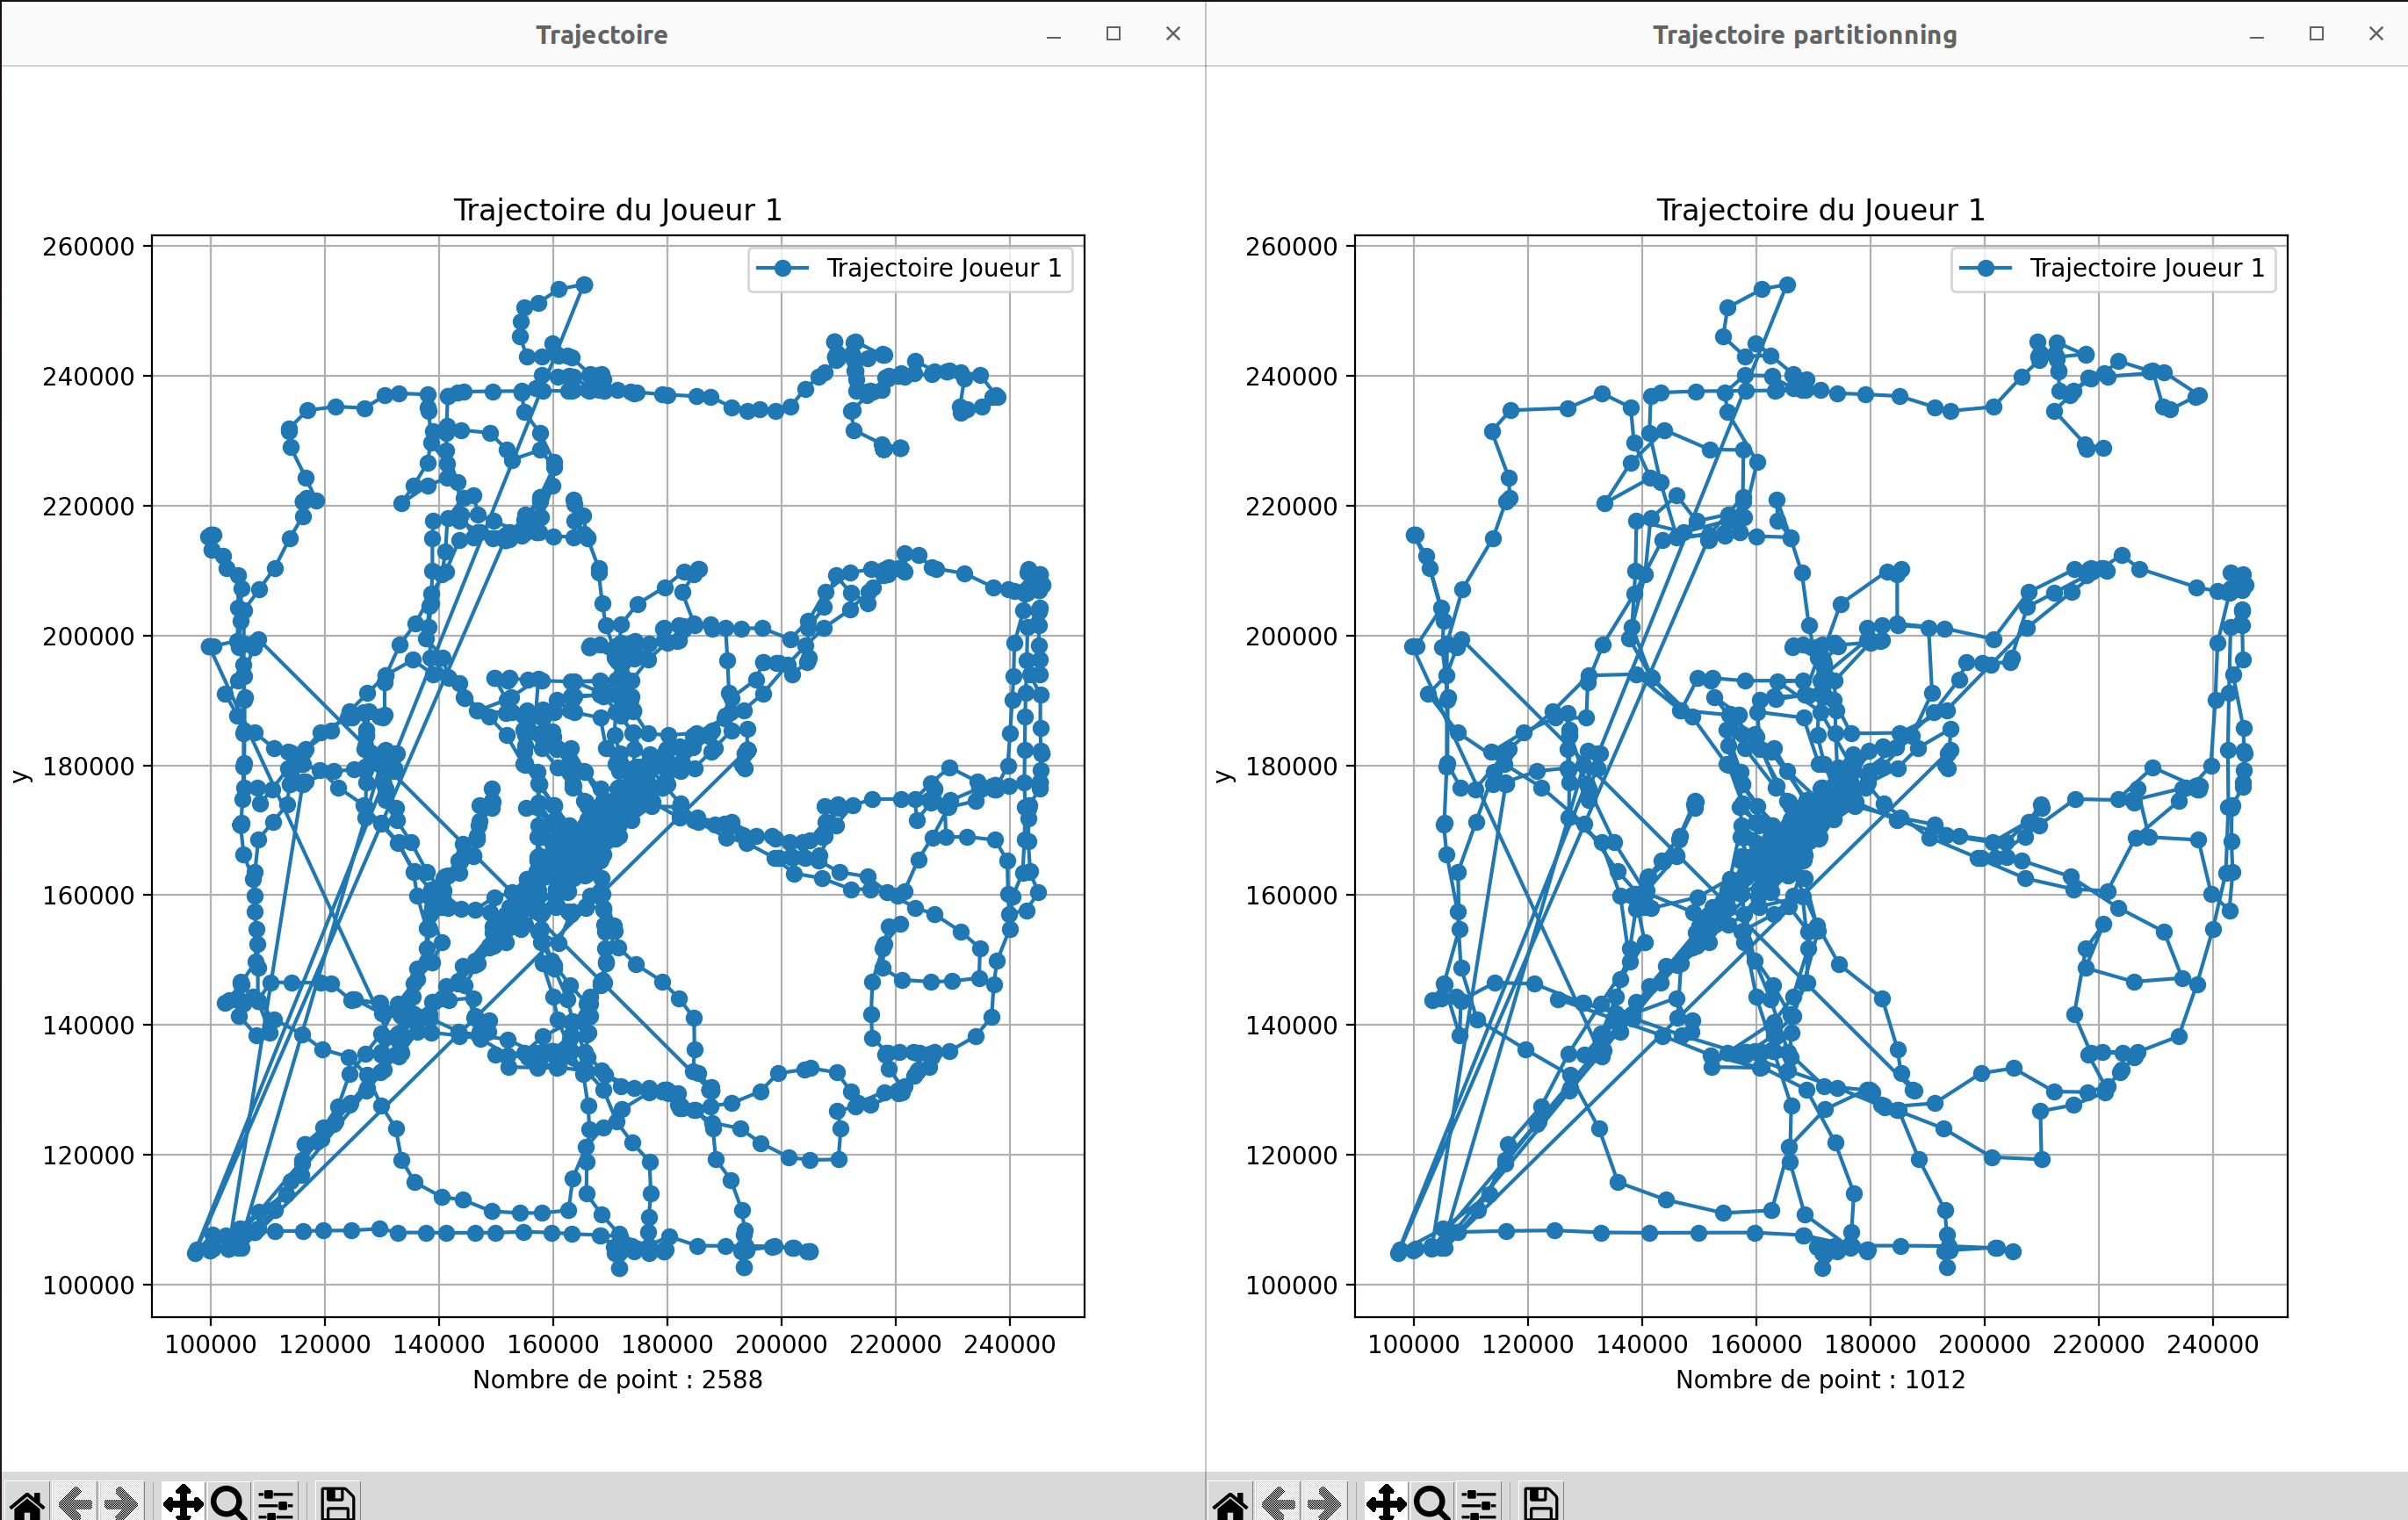
\includegraphics[scale=0.12]{img/etat.png}
            \caption{Graphique complet avant et après l'approche MDL}
            \label{test_mdl}
        \end{figure}

        \begin{figure}[htbp]
            \centering
            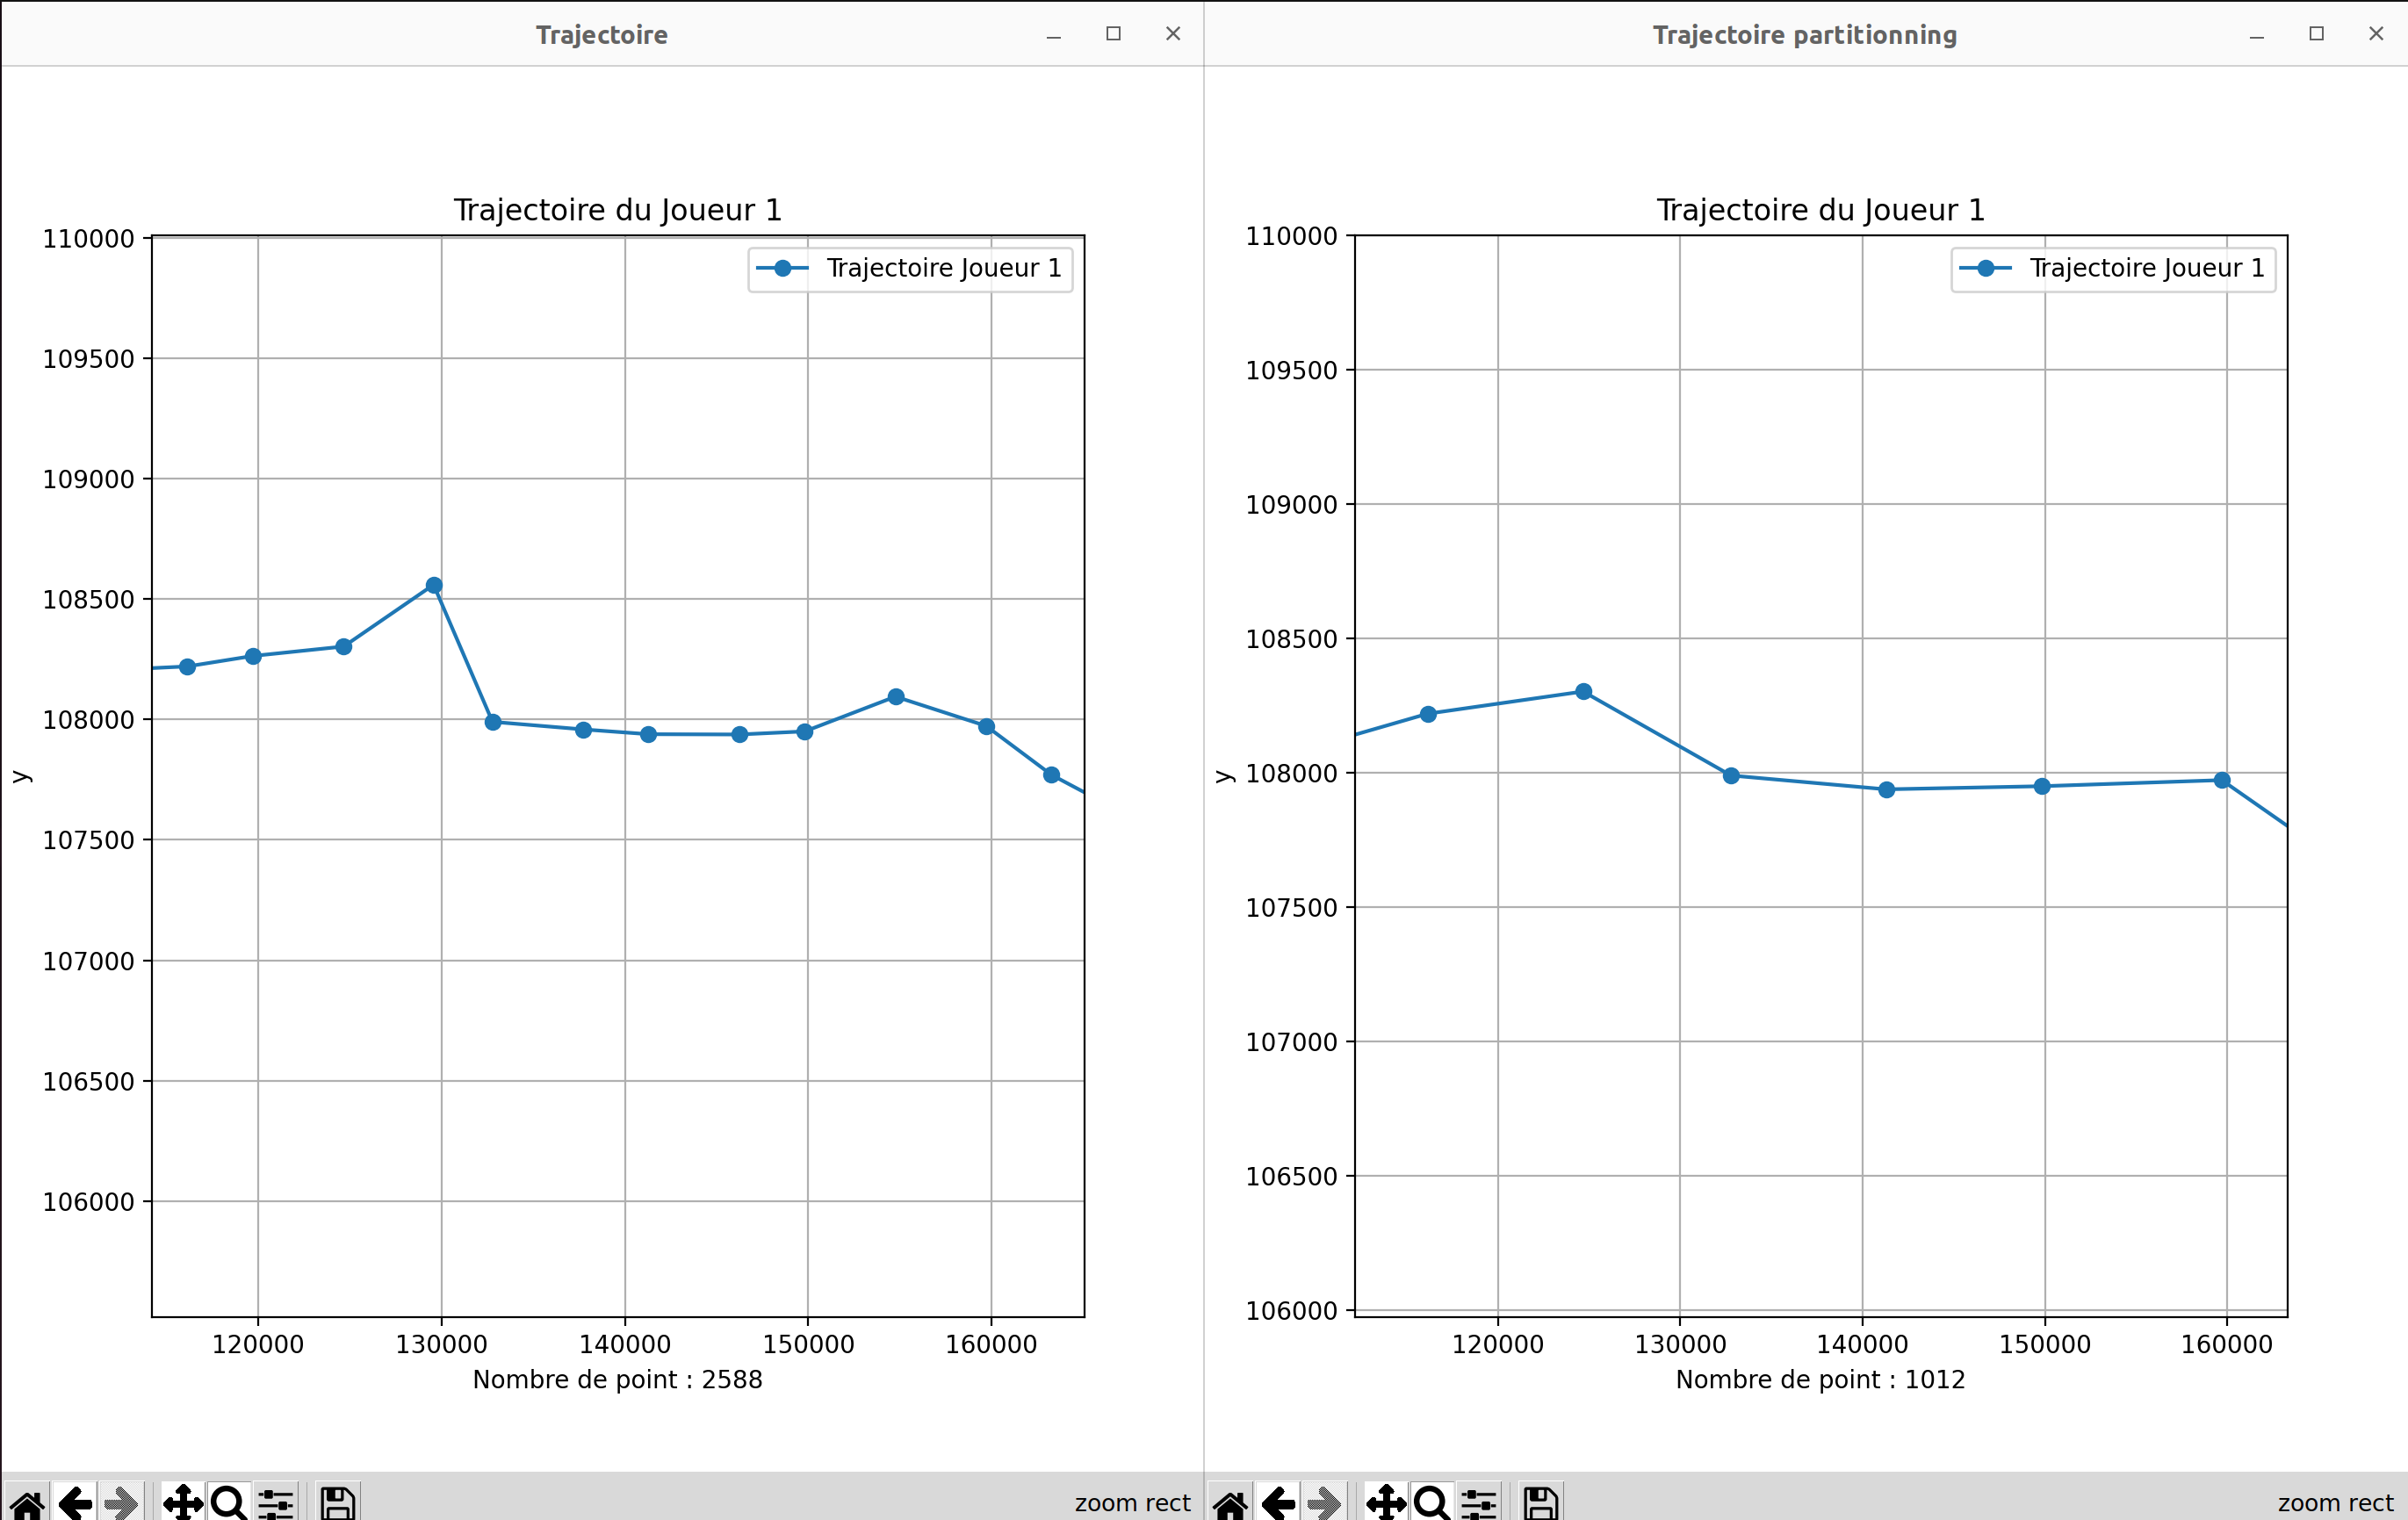
\includegraphics[scale=0.12]{img/etat2.png}
            \caption{Zoom sur une trajectoire avant et après l'approche MDL}
            \label{test_mdl_zoom}
        \end{figure}

    \subsection{Algorithme KMean}
        L’algorithme K-Means est une méthode de partitionnement utilisée pour regrouper des points de données en un ensemble de $k$ clusters. Dans le cadre de l’analyse des trajectoires de joueurs, il permet d’identifier des motifs récurrents de déplacement et de mieux comprendre les stratégies adoptées par les joueurs dans différentes situations.
        
        L’objectif principal de cet algorithme est de regrouper les trajectoires en attribuant chaque point à un cluster dont le centroïde est le plus proche. Cependant, dans notre cas, une adaptation a été nécessaire pour tenir compte de la dimension temporelle des trajectoires. En effet, le facteur temps est un élément crucial dans l’analyse des trajectoires, car un même déplacement peut avoir une signification différente selon le moment où il est effectué.
        
        L’algorithme suit les étapes suivantes :
        
        \begin{enumerate}
            \item Sélection aléatoire de $k$ centroïdes parmi les points de données.
            \item Attribution de chaque point au centroïde le plus proche, en tenant compte de la pondération temporelle.
            \item Mise à jour des centroïdes en calculant la moyenne des points de chaque cluster.
            \item Répétition du processus jusqu’à convergence, c’est-à-dire lorsque les centroïdes ne se déplacent plus significativement.
        \end{enumerate}
        
        L’un des aspects clés de notre implémentation est l’introduction d’une pondération temporelle dans le calcul des distances. En effet, la simple distance euclidienne entre les points $(x, y)$ ne suffit pas à capturer la complexité des trajectoires. Nous avons donc défini une distance pondérée qui prend en compte le facteur temporel pour prendre une valeur entre 0 et 1.
    

        L’initialisation des centroïdes se fait par la sélection aléatoire de $k$ points parmi l’ensemble des données.
        L’algorithme continue ensuite à itérer en attribuant les points aux centroïdes les plus proches et en recalculant les nouveaux centroïdes. Ce processus est répété jusqu’à ce que les centroïdes ne se déplacent plus de manière significative d’une itération à l’autre. Cette condition de convergence est vérifiée en comparant le déplacement moyen des centroïdes avec un seuil de tolérance préalablement défini.\\
        Les clusters ainsi formés permettent d’extraire des caractéristiques pertinentes sur les comportements des joueurs, ouvrant ainsi la voie à des analyses plus poussées et à l’utilisation d’autres algorithmes complémentaires tels que PrefixSpan pour la découverte de motifs séquentiels dans les trajectoires.



        %% Mettre ici une image des clusters

        \begin{algorithm}[H]
            \caption{K-Means pour le clustering des trajectoires}
            \KwIn{$data$: Ensemble de points $(x, y, tick)$,\newline
            $k$: Nombre de clusters,\newline
            $max_iters$: Nombre maximal d'itérations,\newline
            $tol$: Seuil d'arrêt}
            \KwOut{Clusters et centroids optimaux}
            
            \tcc{Initialisation des centroids}
            Sélectionner $k$ points aléatoires de $data$ comme centroids ;
            
            \For{$iteration = 1$ \KwTo $max_iters$}{
            Initialiser $clusters$ comme une liste vide de taille $k$ ;
            
            \tcc{Assignation des points aux centroids les plus proches}
            \ForEach{$point \in data$}{
                Calculer la distance entre $point$ et chaque centroid \;
                Assigner $point$ au cluster du centroid le plus proche \;
            }
            
            \tcc{Mise à jour des centroids}
            \ForEach{$cluster \in clusters$}{
                \If{$cluster$ n'est pas vide}{
                    Calculer le nouveau centroid comme la moyenne des points du cluster \;
                }
            }
            
            \tcc{Vérification de la convergence}
            Calculer le déplacement moyen des centroids \;
            \If{$déplacement < tol$}{
                \textbf{break} \tcp{Arrêt si convergence atteinte}
            }
            
            }
            
            \textbf{Retourner} les clusters et leurs centroids \;
        \end{algorithm}

        \begin{figure}[htbp]
            \centering
            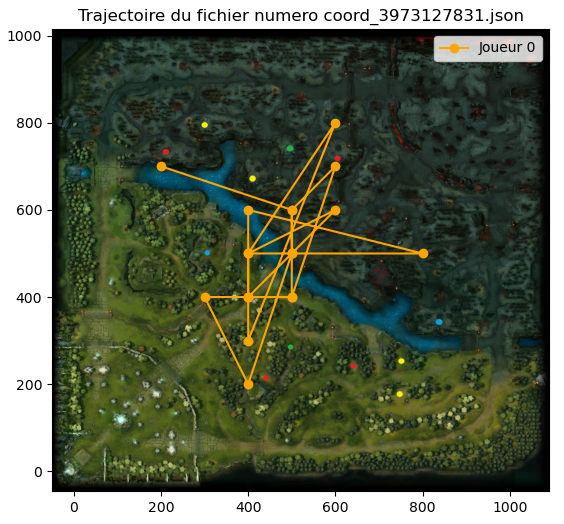
\includegraphics[scale=0.4]{img/example_kmean.png}
            \caption{Segmentation des trajectoires par K-Means}
            \label{test_mdl}
        \end{figure}
        
        \subsection{Algorithme prefixspan}
         PrefixSpan est utilisé pour repérer des motifs de déplacement récurrents parmi les joueurs. L'objectif est d’identifier des suites d’actions qui apparaissent dans un certain pourcentage de parties. Ces suites d'actions peuvent être d'aller à un objectif neutre, ou bien simplement retourner sur sa voie de jeu. Nous avons utilisé un package prédéfini nommé prefixspan.
        

    \section{Architecture du projet}
        \begin{center}
            \resizebox{1.0\textwidth}{!}{% Graphic for TeX using PGF
% Title: /home/faupoin221/Documents/L3/S6/faupoint_doguet_bossu_moalic_dota2/Diagramme1.dia
% Creator: Dia v0.97+git
% CreationDate: Wed Mar 12 12:14:12 2025
% For: faupoin221@CAMPUS
% \usepackage{tikz}
% The following commands are not supported in PSTricks at present
% We define them conditionally, so when they are implemented,
% this pgf file will use them.
\ifx\du\undefined
  \newlength{\du}
\fi
\setlength{\du}{15\unitlength}
\begin{tikzpicture}[even odd rule]
\pgftransformxscale{1.000000}
\pgftransformyscale{-1.000000}
\definecolor{dialinecolor}{rgb}{0.000000, 0.000000, 0.000000}
\pgfsetstrokecolor{dialinecolor}
\pgfsetstrokeopacity{1.000000}
\definecolor{diafillcolor}{rgb}{1.000000, 1.000000, 1.000000}
\pgfsetfillcolor{diafillcolor}
\pgfsetfillopacity{1.000000}
\pgfsetlinewidth{0.100000\du}
\pgfsetdash{}{0pt}
\definecolor{diafillcolor}{rgb}{1.000000, 1.000000, 1.000000}
\pgfsetfillcolor{diafillcolor}
\pgfsetfillopacity{1.000000}
\fill (3.372610\du,4.067850\du)--(8.492610\du,4.067850\du)--(8.492610\du,5.467850\du)--(3.372610\du,5.467850\du)--cycle;
\definecolor{dialinecolor}{rgb}{0.000000, 0.000000, 0.000000}
\pgfsetstrokecolor{dialinecolor}
\pgfsetstrokeopacity{1.000000}
\draw (3.372610\du,4.067850\du)--(8.492610\du,4.067850\du)--(8.492610\du,5.467850\du)--(3.372610\du,5.467850\du)--cycle;
% setfont left to latex
\definecolor{dialinecolor}{rgb}{0.000000, 0.000000, 0.000000}
\pgfsetstrokecolor{dialinecolor}
\pgfsetstrokeopacity{1.000000}
\definecolor{diafillcolor}{rgb}{0.000000, 0.000000, 0.000000}
\pgfsetfillcolor{diafillcolor}
\pgfsetfillopacity{1.000000}
\node[anchor=base,inner sep=0pt, outer sep=0pt,color=dialinecolor] at (5.932610\du,5.010428\du){Point};
\definecolor{diafillcolor}{rgb}{1.000000, 1.000000, 1.000000}
\pgfsetfillcolor{diafillcolor}
\pgfsetfillopacity{1.000000}
\fill (3.372610\du,5.467850\du)--(8.492610\du,5.467850\du)--(8.492610\du,8.067850\du)--(3.372610\du,8.067850\du)--cycle;
\definecolor{dialinecolor}{rgb}{0.000000, 0.000000, 0.000000}
\pgfsetstrokecolor{dialinecolor}
\pgfsetstrokeopacity{1.000000}
\draw (3.372610\du,5.467850\du)--(8.492610\du,5.467850\du)--(8.492610\du,8.067850\du)--(3.372610\du,8.067850\du)--cycle;
% setfont left to latex
\definecolor{dialinecolor}{rgb}{0.000000, 0.000000, 0.000000}
\pgfsetstrokecolor{dialinecolor}
\pgfsetstrokeopacity{1.000000}
\definecolor{diafillcolor}{rgb}{0.000000, 0.000000, 0.000000}
\pgfsetfillcolor{diafillcolor}
\pgfsetfillopacity{1.000000}
\node[anchor=base west,inner sep=0pt,outer sep=0pt,color=dialinecolor] at (3.522610\du,6.161912\du){+x: int};
% setfont left to latex
\definecolor{dialinecolor}{rgb}{0.000000, 0.000000, 0.000000}
\pgfsetstrokecolor{dialinecolor}
\pgfsetstrokeopacity{1.000000}
\definecolor{diafillcolor}{rgb}{0.000000, 0.000000, 0.000000}
\pgfsetfillcolor{diafillcolor}
\pgfsetfillopacity{1.000000}
\node[anchor=base west,inner sep=0pt,outer sep=0pt,color=dialinecolor] at (3.522610\du,6.961912\du){+y: int};
% setfont left to latex
\definecolor{dialinecolor}{rgb}{0.000000, 0.000000, 0.000000}
\pgfsetstrokecolor{dialinecolor}
\pgfsetstrokeopacity{1.000000}
\definecolor{diafillcolor}{rgb}{0.000000, 0.000000, 0.000000}
\pgfsetfillcolor{diafillcolor}
\pgfsetfillopacity{1.000000}
\node[anchor=base west,inner sep=0pt,outer sep=0pt,color=dialinecolor] at (3.522610\du,7.761912\du){+tick: int};
\definecolor{diafillcolor}{rgb}{1.000000, 1.000000, 1.000000}
\pgfsetfillcolor{diafillcolor}
\pgfsetfillopacity{1.000000}
\fill (3.372610\du,8.067850\du)--(8.492610\du,8.067850\du)--(8.492610\du,9.867850\du)--(3.372610\du,9.867850\du)--cycle;
\definecolor{dialinecolor}{rgb}{0.000000, 0.000000, 0.000000}
\pgfsetstrokecolor{dialinecolor}
\pgfsetstrokeopacity{1.000000}
\draw (3.372610\du,8.067850\du)--(8.492610\du,8.067850\du)--(8.492610\du,9.867850\du)--(3.372610\du,9.867850\du)--cycle;
% setfont left to latex
\definecolor{dialinecolor}{rgb}{0.000000, 0.000000, 0.000000}
\pgfsetstrokecolor{dialinecolor}
\pgfsetstrokeopacity{1.000000}
\definecolor{diafillcolor}{rgb}{0.000000, 0.000000, 0.000000}
\pgfsetfillcolor{diafillcolor}
\pgfsetfillopacity{1.000000}
\node[anchor=base west,inner sep=0pt,outer sep=0pt,color=dialinecolor] at (3.522610\du,8.761912\du){+get\_coord()};
% setfont left to latex
\definecolor{dialinecolor}{rgb}{0.000000, 0.000000, 0.000000}
\pgfsetstrokecolor{dialinecolor}
\pgfsetstrokeopacity{1.000000}
\definecolor{diafillcolor}{rgb}{0.000000, 0.000000, 0.000000}
\pgfsetfillcolor{diafillcolor}
\pgfsetfillopacity{1.000000}
\node[anchor=base west,inner sep=0pt,outer sep=0pt,color=dialinecolor] at (3.522610\du,9.561912\du){+get\_tick()};
\pgfsetlinewidth{0.100000\du}
\pgfsetdash{}{0pt}
\definecolor{diafillcolor}{rgb}{1.000000, 1.000000, 1.000000}
\pgfsetfillcolor{diafillcolor}
\pgfsetfillopacity{1.000000}
\fill (-0.547560\du,-7.222500\du)--(8.807440\du,-7.222500\du)--(8.807440\du,-5.822500\du)--(-0.547560\du,-5.822500\du)--cycle;
\definecolor{dialinecolor}{rgb}{0.000000, 0.000000, 0.000000}
\pgfsetstrokecolor{dialinecolor}
\pgfsetstrokeopacity{1.000000}
\draw (-0.547560\du,-7.222500\du)--(8.807440\du,-7.222500\du)--(8.807440\du,-5.822500\du)--(-0.547560\du,-5.822500\du)--cycle;
% setfont left to latex
\definecolor{dialinecolor}{rgb}{0.000000, 0.000000, 0.000000}
\pgfsetstrokecolor{dialinecolor}
\pgfsetstrokeopacity{1.000000}
\definecolor{diafillcolor}{rgb}{0.000000, 0.000000, 0.000000}
\pgfsetfillcolor{diafillcolor}
\pgfsetfillopacity{1.000000}
\node[anchor=base,inner sep=0pt, outer sep=0pt,color=dialinecolor] at (4.129940\du,-6.279922\du){Trajectoire};
\definecolor{diafillcolor}{rgb}{1.000000, 1.000000, 1.000000}
\pgfsetfillcolor{diafillcolor}
\pgfsetfillopacity{1.000000}
\fill (-0.547560\du,-5.822500\du)--(8.807440\du,-5.822500\du)--(8.807440\du,-4.022500\du)--(-0.547560\du,-4.022500\du)--cycle;
\definecolor{dialinecolor}{rgb}{0.000000, 0.000000, 0.000000}
\pgfsetstrokecolor{dialinecolor}
\pgfsetstrokeopacity{1.000000}
\draw (-0.547560\du,-5.822500\du)--(8.807440\du,-5.822500\du)--(8.807440\du,-4.022500\du)--(-0.547560\du,-4.022500\du)--cycle;
% setfont left to latex
\definecolor{dialinecolor}{rgb}{0.000000, 0.000000, 0.000000}
\pgfsetstrokecolor{dialinecolor}
\pgfsetstrokeopacity{1.000000}
\definecolor{diafillcolor}{rgb}{0.000000, 0.000000, 0.000000}
\pgfsetfillcolor{diafillcolor}
\pgfsetfillopacity{1.000000}
\node[anchor=base west,inner sep=0pt,outer sep=0pt,color=dialinecolor] at (-0.397560\du,-5.128438\du){+player\_id: int};
% setfont left to latex
\definecolor{dialinecolor}{rgb}{0.000000, 0.000000, 0.000000}
\pgfsetstrokecolor{dialinecolor}
\pgfsetstrokeopacity{1.000000}
\definecolor{diafillcolor}{rgb}{0.000000, 0.000000, 0.000000}
\pgfsetfillcolor{diafillcolor}
\pgfsetfillopacity{1.000000}
\node[anchor=base west,inner sep=0pt,outer sep=0pt,color=dialinecolor] at (-0.397560\du,-4.328438\du){+points: Point};
\definecolor{diafillcolor}{rgb}{1.000000, 1.000000, 1.000000}
\pgfsetfillcolor{diafillcolor}
\pgfsetfillopacity{1.000000}
\fill (-0.547560\du,-4.022500\du)--(8.807440\du,-4.022500\du)--(8.807440\du,0.177500\du)--(-0.547560\du,0.177500\du)--cycle;
\definecolor{dialinecolor}{rgb}{0.000000, 0.000000, 0.000000}
\pgfsetstrokecolor{dialinecolor}
\pgfsetstrokeopacity{1.000000}
\draw (-0.547560\du,-4.022500\du)--(8.807440\du,-4.022500\du)--(8.807440\du,0.177500\du)--(-0.547560\du,0.177500\du)--cycle;
% setfont left to latex
\definecolor{dialinecolor}{rgb}{0.000000, 0.000000, 0.000000}
\pgfsetstrokecolor{dialinecolor}
\pgfsetstrokeopacity{1.000000}
\definecolor{diafillcolor}{rgb}{0.000000, 0.000000, 0.000000}
\pgfsetfillcolor{diafillcolor}
\pgfsetfillopacity{1.000000}
\node[anchor=base west,inner sep=0pt,outer sep=0pt,color=dialinecolor] at (-0.397560\du,-3.328437\du){+sub\_trajectories()};
% setfont left to latex
\definecolor{dialinecolor}{rgb}{0.000000, 0.000000, 0.000000}
\pgfsetstrokecolor{dialinecolor}
\pgfsetstrokeopacity{1.000000}
\definecolor{diafillcolor}{rgb}{0.000000, 0.000000, 0.000000}
\pgfsetfillcolor{diafillcolor}
\pgfsetfillopacity{1.000000}
\node[anchor=base west,inner sep=0pt,outer sep=0pt,color=dialinecolor] at (-0.397560\du,-2.528437\du){+get\_partial\_segments()};
% setfont left to latex
\definecolor{dialinecolor}{rgb}{0.000000, 0.000000, 0.000000}
\pgfsetstrokecolor{dialinecolor}
\pgfsetstrokeopacity{1.000000}
\definecolor{diafillcolor}{rgb}{0.000000, 0.000000, 0.000000}
\pgfsetfillcolor{diafillcolor}
\pgfsetfillopacity{1.000000}
\node[anchor=base west,inner sep=0pt,outer sep=0pt,color=dialinecolor] at (-0.397560\du,-1.728437\du){+get\_segments()};
% setfont left to latex
\definecolor{dialinecolor}{rgb}{0.000000, 0.000000, 0.000000}
\pgfsetstrokecolor{dialinecolor}
\pgfsetstrokeopacity{1.000000}
\definecolor{diafillcolor}{rgb}{0.000000, 0.000000, 0.000000}
\pgfsetfillcolor{diafillcolor}
\pgfsetfillopacity{1.000000}
\node[anchor=base west,inner sep=0pt,outer sep=0pt,color=dialinecolor] at (-0.397560\du,-0.928437\du){+get\_point()};
% setfont left to latex
\definecolor{dialinecolor}{rgb}{0.000000, 0.000000, 0.000000}
\pgfsetstrokecolor{dialinecolor}
\pgfsetstrokeopacity{1.000000}
\definecolor{diafillcolor}{rgb}{0.000000, 0.000000, 0.000000}
\pgfsetfillcolor{diafillcolor}
\pgfsetfillopacity{1.000000}
\node[anchor=base west,inner sep=0pt,outer sep=0pt,color=dialinecolor] at (-0.397560\du,-0.128437\du){+get\_all\_points()};
\pgfsetlinewidth{0.100000\du}
\pgfsetdash{}{0pt}
\definecolor{diafillcolor}{rgb}{1.000000, 1.000000, 1.000000}
\pgfsetfillcolor{diafillcolor}
\pgfsetfillopacity{1.000000}
\fill (-4.812250\du,13.255100\du)--(16.477750\du,13.255100\du)--(16.477750\du,14.655100\du)--(-4.812250\du,14.655100\du)--cycle;
\definecolor{dialinecolor}{rgb}{0.000000, 0.000000, 0.000000}
\pgfsetstrokecolor{dialinecolor}
\pgfsetstrokeopacity{1.000000}
\draw (-4.812250\du,13.255100\du)--(16.477750\du,13.255100\du)--(16.477750\du,14.655100\du)--(-4.812250\du,14.655100\du)--cycle;
% setfont left to latex
\definecolor{dialinecolor}{rgb}{0.000000, 0.000000, 0.000000}
\pgfsetstrokecolor{dialinecolor}
\pgfsetstrokeopacity{1.000000}
\definecolor{diafillcolor}{rgb}{0.000000, 0.000000, 0.000000}
\pgfsetfillcolor{diafillcolor}
\pgfsetfillopacity{1.000000}
\node[anchor=base,inner sep=0pt, outer sep=0pt,color=dialinecolor] at (5.832750\du,14.197678\du){data\_manager};
\definecolor{diafillcolor}{rgb}{1.000000, 1.000000, 1.000000}
\pgfsetfillcolor{diafillcolor}
\pgfsetfillopacity{1.000000}
\fill (-4.812250\du,14.655100\du)--(16.477750\du,14.655100\du)--(16.477750\du,15.055100\du)--(-4.812250\du,15.055100\du)--cycle;
\definecolor{dialinecolor}{rgb}{0.000000, 0.000000, 0.000000}
\pgfsetstrokecolor{dialinecolor}
\pgfsetstrokeopacity{1.000000}
\draw (-4.812250\du,14.655100\du)--(16.477750\du,14.655100\du)--(16.477750\du,15.055100\du)--(-4.812250\du,15.055100\du)--cycle;
\definecolor{diafillcolor}{rgb}{1.000000, 1.000000, 1.000000}
\pgfsetfillcolor{diafillcolor}
\pgfsetfillopacity{1.000000}
\fill (-4.812250\du,15.055100\du)--(16.477750\du,15.055100\du)--(16.477750\du,20.855100\du)--(-4.812250\du,20.855100\du)--cycle;
\definecolor{dialinecolor}{rgb}{0.000000, 0.000000, 0.000000}
\pgfsetstrokecolor{dialinecolor}
\pgfsetstrokeopacity{1.000000}
\draw (-4.812250\du,15.055100\du)--(16.477750\du,15.055100\du)--(16.477750\du,20.855100\du)--(-4.812250\du,20.855100\du)--cycle;
% setfont left to latex
\definecolor{dialinecolor}{rgb}{0.000000, 0.000000, 0.000000}
\pgfsetstrokecolor{dialinecolor}
\pgfsetstrokeopacity{1.000000}
\definecolor{diafillcolor}{rgb}{0.000000, 0.000000, 0.000000}
\pgfsetfillcolor{diafillcolor}
\pgfsetfillopacity{1.000000}
\node[anchor=base west,inner sep=0pt,outer sep=0pt,color=dialinecolor] at (-4.662250\du,15.749163\du){+\_create\_point(x,y,tick,vec\_x,vec\_y,min\_max\_values)};
% setfont left to latex
\definecolor{dialinecolor}{rgb}{0.000000, 0.000000, 0.000000}
\pgfsetstrokecolor{dialinecolor}
\pgfsetstrokeopacity{1.000000}
\definecolor{diafillcolor}{rgb}{0.000000, 0.000000, 0.000000}
\pgfsetfillcolor{diafillcolor}
\pgfsetfillopacity{1.000000}
\node[anchor=base west,inner sep=0pt,outer sep=0pt,color=dialinecolor] at (-4.662250\du,16.549163\du){+\_find\_min\_max(data)};
% setfont left to latex
\definecolor{dialinecolor}{rgb}{0.000000, 0.000000, 0.000000}
\pgfsetstrokecolor{dialinecolor}
\pgfsetstrokeopacity{1.000000}
\definecolor{diafillcolor}{rgb}{0.000000, 0.000000, 0.000000}
\pgfsetfillcolor{diafillcolor}
\pgfsetfillopacity{1.000000}
\node[anchor=base west,inner sep=0pt,outer sep=0pt,color=dialinecolor] at (-4.662250\du,17.349163\du){+load\_data\_from\_csv(file\_path:str)};
% setfont left to latex
\definecolor{dialinecolor}{rgb}{0.000000, 0.000000, 0.000000}
\pgfsetstrokecolor{dialinecolor}
\pgfsetstrokeopacity{1.000000}
\definecolor{diafillcolor}{rgb}{0.000000, 0.000000, 0.000000}
\pgfsetfillcolor{diafillcolor}
\pgfsetfillopacity{1.000000}
\node[anchor=base west,inner sep=0pt,outer sep=0pt,color=dialinecolor] at (-4.662250\du,18.149163\du){+export\_trajectories\_to\_json(trajectoires:Trajectoire,};
\definecolor{dialinecolor}{rgb}{0.000000, 0.000000, 0.000000}
\pgfsetstrokecolor{dialinecolor}
\pgfsetstrokeopacity{1.000000}
\definecolor{diafillcolor}{rgb}{0.000000, 0.000000, 0.000000}
\pgfsetfillcolor{diafillcolor}
\pgfsetfillopacity{1.000000}
\node[anchor=base west,inner sep=0pt,outer sep=0pt,color=dialinecolor] at (-4.662250\du,18.949163\du){                             file\_path:str)};
% setfont left to latex
\definecolor{dialinecolor}{rgb}{0.000000, 0.000000, 0.000000}
\pgfsetstrokecolor{dialinecolor}
\pgfsetstrokeopacity{1.000000}
\definecolor{diafillcolor}{rgb}{0.000000, 0.000000, 0.000000}
\pgfsetfillcolor{diafillcolor}
\pgfsetfillopacity{1.000000}
\node[anchor=base west,inner sep=0pt,outer sep=0pt,color=dialinecolor] at (-4.662250\du,19.749163\du){+load\_traj\_from\_json(file\_path:str)};
% setfont left to latex
\definecolor{dialinecolor}{rgb}{0.000000, 0.000000, 0.000000}
\pgfsetstrokecolor{dialinecolor}
\pgfsetstrokeopacity{1.000000}
\definecolor{diafillcolor}{rgb}{0.000000, 0.000000, 0.000000}
\pgfsetfillcolor{diafillcolor}
\pgfsetfillopacity{1.000000}
\node[anchor=base west,inner sep=0pt,outer sep=0pt,color=dialinecolor] at (-4.662250\du,20.549163\du){+()};
\pgfsetlinewidth{0.100000\du}
\pgfsetdash{{0.400000\du}{0.400000\du}}{0\du}
\pgfsetmiterjoin
\pgfsetbuttcap
{
\definecolor{diafillcolor}{rgb}{0.000000, 0.000000, 0.000000}
\pgfsetfillcolor{diafillcolor}
\pgfsetfillopacity{1.000000}
% was here!!!
\definecolor{dialinecolor}{rgb}{0.000000, 0.000000, 0.000000}
\pgfsetstrokecolor{dialinecolor}
\pgfsetstrokeopacity{1.000000}
\draw (4.129940\du,0.177500\du)--(4.129940\du,2.522675\du)--(5.932610\du,2.522675\du)--(5.932610\du,4.067850\du);
}
\definecolor{dialinecolor}{rgb}{0.000000, 0.000000, 0.000000}
\pgfsetstrokecolor{dialinecolor}
\pgfsetstrokeopacity{1.000000}
\draw (4.129940\du,1.089303\du)--(4.129940\du,2.522675\du)--(5.932610\du,2.522675\du)--(5.932610\du,4.067850\du);
\pgfsetlinewidth{0.100000\du}
\pgfsetdash{}{0pt}
\pgfsetmiterjoin
\definecolor{diafillcolor}{rgb}{1.000000, 1.000000, 1.000000}
\pgfsetfillcolor{diafillcolor}
\pgfsetfillopacity{1.000000}
\fill (4.529940\du,1.089303\du)--(4.129940\du,0.289303\du)--(3.729940\du,1.089303\du)--cycle;
\definecolor{dialinecolor}{rgb}{0.000000, 0.000000, 0.000000}
\pgfsetstrokecolor{dialinecolor}
\pgfsetstrokeopacity{1.000000}
\draw (4.529940\du,1.089303\du)--(4.129940\du,0.289303\du)--(3.729940\du,1.089303\du)--cycle;
% setfont left to latex
\pgfsetlinewidth{0.100000\du}
\pgfsetdash{{0.400000\du}{0.400000\du}}{0\du}
\pgfsetmiterjoin
\pgfsetbuttcap
{
\definecolor{diafillcolor}{rgb}{0.000000, 0.000000, 0.000000}
\pgfsetfillcolor{diafillcolor}
\pgfsetfillopacity{1.000000}
% was here!!!
\definecolor{dialinecolor}{rgb}{0.000000, 0.000000, 0.000000}
\pgfsetstrokecolor{dialinecolor}
\pgfsetstrokeopacity{1.000000}
\draw (5.932610\du,9.867850\du)--(5.932610\du,11.961475\du)--(5.832750\du,11.961475\du)--(5.832750\du,13.255100\du);
}
\definecolor{dialinecolor}{rgb}{0.000000, 0.000000, 0.000000}
\pgfsetstrokecolor{dialinecolor}
\pgfsetstrokeopacity{1.000000}
\draw (5.932610\du,10.779653\du)--(5.932610\du,11.961475\du)--(5.832750\du,11.961475\du)--(5.832750\du,13.255100\du);
\pgfsetlinewidth{0.100000\du}
\pgfsetdash{}{0pt}
\pgfsetmiterjoin
\definecolor{diafillcolor}{rgb}{1.000000, 1.000000, 1.000000}
\pgfsetfillcolor{diafillcolor}
\pgfsetfillopacity{1.000000}
\fill (6.332610\du,10.779653\du)--(5.932610\du,9.979653\du)--(5.532610\du,10.779653\du)--cycle;
\definecolor{dialinecolor}{rgb}{0.000000, 0.000000, 0.000000}
\pgfsetstrokecolor{dialinecolor}
\pgfsetstrokeopacity{1.000000}
\draw (6.332610\du,10.779653\du)--(5.932610\du,9.979653\du)--(5.532610\du,10.779653\du)--cycle;
% setfont left to latex
\pgfsetlinewidth{0.100000\du}
\pgfsetdash{}{0pt}
\definecolor{diafillcolor}{rgb}{1.000000, 1.000000, 1.000000}
\pgfsetfillcolor{diafillcolor}
\pgfsetfillopacity{1.000000}
\fill (13.844200\du,-19.869600\du)--(37.444200\du,-19.869600\du)--(37.444200\du,-18.469600\du)--(13.844200\du,-18.469600\du)--cycle;
\definecolor{dialinecolor}{rgb}{0.000000, 0.000000, 0.000000}
\pgfsetstrokecolor{dialinecolor}
\pgfsetstrokeopacity{1.000000}
\draw (13.844200\du,-19.869600\du)--(37.444200\du,-19.869600\du)--(37.444200\du,-18.469600\du)--(13.844200\du,-18.469600\du)--cycle;
% setfont left to latex
\definecolor{dialinecolor}{rgb}{0.000000, 0.000000, 0.000000}
\pgfsetstrokecolor{dialinecolor}
\pgfsetstrokeopacity{1.000000}
\definecolor{diafillcolor}{rgb}{0.000000, 0.000000, 0.000000}
\pgfsetfillcolor{diafillcolor}
\pgfsetfillopacity{1.000000}
\node[anchor=base,inner sep=0pt, outer sep=0pt,color=dialinecolor] at (25.644200\du,-18.927022\du){KMeans};
\definecolor{diafillcolor}{rgb}{1.000000, 1.000000, 1.000000}
\pgfsetfillcolor{diafillcolor}
\pgfsetfillopacity{1.000000}
\fill (13.844200\du,-18.469600\du)--(37.444200\du,-18.469600\du)--(37.444200\du,-13.469600\du)--(13.844200\du,-13.469600\du)--cycle;
\definecolor{dialinecolor}{rgb}{0.000000, 0.000000, 0.000000}
\pgfsetstrokecolor{dialinecolor}
\pgfsetstrokeopacity{1.000000}
\draw (13.844200\du,-18.469600\du)--(37.444200\du,-18.469600\du)--(37.444200\du,-13.469600\du)--(13.844200\du,-13.469600\du)--cycle;
% setfont left to latex
\definecolor{dialinecolor}{rgb}{0.000000, 0.000000, 0.000000}
\pgfsetstrokecolor{dialinecolor}
\pgfsetstrokeopacity{1.000000}
\definecolor{diafillcolor}{rgb}{0.000000, 0.000000, 0.000000}
\pgfsetfillcolor{diafillcolor}
\pgfsetfillopacity{1.000000}
\node[anchor=base west,inner sep=0pt,outer sep=0pt,color=dialinecolor] at (13.994200\du,-17.775537\du){+k: int};
% setfont left to latex
\definecolor{dialinecolor}{rgb}{0.000000, 0.000000, 0.000000}
\pgfsetstrokecolor{dialinecolor}
\pgfsetstrokeopacity{1.000000}
\definecolor{diafillcolor}{rgb}{0.000000, 0.000000, 0.000000}
\pgfsetfillcolor{diafillcolor}
\pgfsetfillopacity{1.000000}
\node[anchor=base west,inner sep=0pt,outer sep=0pt,color=dialinecolor] at (13.994200\du,-16.975537\du){+max\_iters: int};
% setfont left to latex
\definecolor{dialinecolor}{rgb}{0.000000, 0.000000, 0.000000}
\pgfsetstrokecolor{dialinecolor}
\pgfsetstrokeopacity{1.000000}
\definecolor{diafillcolor}{rgb}{0.000000, 0.000000, 0.000000}
\pgfsetfillcolor{diafillcolor}
\pgfsetfillopacity{1.000000}
\node[anchor=base west,inner sep=0pt,outer sep=0pt,color=dialinecolor] at (13.994200\du,-16.175537\du){+time\_weight: float};
% setfont left to latex
\definecolor{dialinecolor}{rgb}{0.000000, 0.000000, 0.000000}
\pgfsetstrokecolor{dialinecolor}
\pgfsetstrokeopacity{1.000000}
\definecolor{diafillcolor}{rgb}{0.000000, 0.000000, 0.000000}
\pgfsetfillcolor{diafillcolor}
\pgfsetfillopacity{1.000000}
\node[anchor=base west,inner sep=0pt,outer sep=0pt,color=dialinecolor] at (13.994200\du,-15.375537\du){+tol: float};
% setfont left to latex
\definecolor{dialinecolor}{rgb}{0.000000, 0.000000, 0.000000}
\pgfsetstrokecolor{dialinecolor}
\pgfsetstrokeopacity{1.000000}
\definecolor{diafillcolor}{rgb}{0.000000, 0.000000, 0.000000}
\pgfsetfillcolor{diafillcolor}
\pgfsetfillopacity{1.000000}
\node[anchor=base west,inner sep=0pt,outer sep=0pt,color=dialinecolor] at (13.994200\du,-14.575537\du){+centroids: list};
% setfont left to latex
\definecolor{dialinecolor}{rgb}{0.000000, 0.000000, 0.000000}
\pgfsetstrokecolor{dialinecolor}
\pgfsetstrokeopacity{1.000000}
\definecolor{diafillcolor}{rgb}{0.000000, 0.000000, 0.000000}
\pgfsetfillcolor{diafillcolor}
\pgfsetfillopacity{1.000000}
\node[anchor=base west,inner sep=0pt,outer sep=0pt,color=dialinecolor] at (13.994200\du,-13.775538\du){+clusters: list};
\definecolor{diafillcolor}{rgb}{1.000000, 1.000000, 1.000000}
\pgfsetfillcolor{diafillcolor}
\pgfsetfillopacity{1.000000}
\fill (13.844200\du,-13.469600\du)--(37.444200\du,-13.469600\du)--(37.444200\du,-8.469600\du)--(13.844200\du,-8.469600\du)--cycle;
\definecolor{dialinecolor}{rgb}{0.000000, 0.000000, 0.000000}
\pgfsetstrokecolor{dialinecolor}
\pgfsetstrokeopacity{1.000000}
\draw (13.844200\du,-13.469600\du)--(37.444200\du,-13.469600\du)--(37.444200\du,-8.469600\du)--(13.844200\du,-8.469600\du)--cycle;
% setfont left to latex
\definecolor{dialinecolor}{rgb}{0.000000, 0.000000, 0.000000}
\pgfsetstrokecolor{dialinecolor}
\pgfsetstrokeopacity{1.000000}
\definecolor{diafillcolor}{rgb}{0.000000, 0.000000, 0.000000}
\pgfsetfillcolor{diafillcolor}
\pgfsetfillopacity{1.000000}
\node[anchor=base west,inner sep=0pt,outer sep=0pt,color=dialinecolor] at (13.994200\du,-12.775538\du){+\_\_init\_\_(k:int=100,max\_iters:int=100,time\_weight:float=0.5,};
\definecolor{dialinecolor}{rgb}{0.000000, 0.000000, 0.000000}
\pgfsetstrokecolor{dialinecolor}
\pgfsetstrokeopacity{1.000000}
\definecolor{diafillcolor}{rgb}{0.000000, 0.000000, 0.000000}
\pgfsetfillcolor{diafillcolor}
\pgfsetfillopacity{1.000000}
\node[anchor=base west,inner sep=0pt,outer sep=0pt,color=dialinecolor] at (13.994200\du,-11.975537\du){          tol:float=1e-4)};
% setfont left to latex
\definecolor{dialinecolor}{rgb}{0.000000, 0.000000, 0.000000}
\pgfsetstrokecolor{dialinecolor}
\pgfsetstrokeopacity{1.000000}
\definecolor{diafillcolor}{rgb}{0.000000, 0.000000, 0.000000}
\pgfsetfillcolor{diafillcolor}
\pgfsetfillopacity{1.000000}
\node[anchor=base west,inner sep=0pt,outer sep=0pt,color=dialinecolor] at (13.994200\du,-11.175538\du){+\_weighted\_distance(p1,p2:tuple)};
% setfont left to latex
\definecolor{dialinecolor}{rgb}{0.000000, 0.000000, 0.000000}
\pgfsetstrokecolor{dialinecolor}
\pgfsetstrokeopacity{1.000000}
\definecolor{diafillcolor}{rgb}{0.000000, 0.000000, 0.000000}
\pgfsetfillcolor{diafillcolor}
\pgfsetfillopacity{1.000000}
\node[anchor=base west,inner sep=0pt,outer sep=0pt,color=dialinecolor] at (13.994200\du,-10.375538\du){+fit(data:list)};
% setfont left to latex
\definecolor{dialinecolor}{rgb}{0.000000, 0.000000, 0.000000}
\pgfsetstrokecolor{dialinecolor}
\pgfsetstrokeopacity{1.000000}
\definecolor{diafillcolor}{rgb}{0.000000, 0.000000, 0.000000}
\pgfsetfillcolor{diafillcolor}
\pgfsetfillopacity{1.000000}
\node[anchor=base west,inner sep=0pt,outer sep=0pt,color=dialinecolor] at (13.994200\du,-9.575538\du){+predict(points:list)};
% setfont left to latex
\definecolor{dialinecolor}{rgb}{0.000000, 0.000000, 0.000000}
\pgfsetstrokecolor{dialinecolor}
\pgfsetstrokeopacity{1.000000}
\definecolor{diafillcolor}{rgb}{0.000000, 0.000000, 0.000000}
\pgfsetfillcolor{diafillcolor}
\pgfsetfillopacity{1.000000}
\node[anchor=base west,inner sep=0pt,outer sep=0pt,color=dialinecolor] at (13.994200\du,-8.775538\du){+prepare\_data\_for\_prefixspan()};
\pgfsetlinewidth{0.100000\du}
\pgfsetdash{}{0pt}
\definecolor{diafillcolor}{rgb}{1.000000, 1.000000, 1.000000}
\pgfsetfillcolor{diafillcolor}
\pgfsetfillopacity{1.000000}
\fill (-14.030500\du,-17.387300\du)--(5.719500\du,-17.387300\du)--(5.719500\du,-15.987300\du)--(-14.030500\du,-15.987300\du)--cycle;
\definecolor{dialinecolor}{rgb}{0.000000, 0.000000, 0.000000}
\pgfsetstrokecolor{dialinecolor}
\pgfsetstrokeopacity{1.000000}
\draw (-14.030500\du,-17.387300\du)--(5.719500\du,-17.387300\du)--(5.719500\du,-15.987300\du)--(-14.030500\du,-15.987300\du)--cycle;
% setfont left to latex
\definecolor{dialinecolor}{rgb}{0.000000, 0.000000, 0.000000}
\pgfsetstrokecolor{dialinecolor}
\pgfsetstrokeopacity{1.000000}
\definecolor{diafillcolor}{rgb}{0.000000, 0.000000, 0.000000}
\pgfsetfillcolor{diafillcolor}
\pgfsetfillopacity{1.000000}
\node[anchor=base,inner sep=0pt, outer sep=0pt,color=dialinecolor] at (-4.155500\du,-16.444722\du){MDL};
\definecolor{diafillcolor}{rgb}{1.000000, 1.000000, 1.000000}
\pgfsetfillcolor{diafillcolor}
\pgfsetfillopacity{1.000000}
\fill (-14.030500\du,-15.987300\du)--(5.719500\du,-15.987300\du)--(5.719500\du,-15.587300\du)--(-14.030500\du,-15.587300\du)--cycle;
\definecolor{dialinecolor}{rgb}{0.000000, 0.000000, 0.000000}
\pgfsetstrokecolor{dialinecolor}
\pgfsetstrokeopacity{1.000000}
\draw (-14.030500\du,-15.987300\du)--(5.719500\du,-15.987300\du)--(5.719500\du,-15.587300\du)--(-14.030500\du,-15.587300\du)--cycle;
\definecolor{diafillcolor}{rgb}{1.000000, 1.000000, 1.000000}
\pgfsetfillcolor{diafillcolor}
\pgfsetfillopacity{1.000000}
\fill (-14.030500\du,-15.587300\du)--(5.719500\du,-15.587300\du)--(5.719500\du,-10.587300\du)--(-14.030500\du,-10.587300\du)--cycle;
\definecolor{dialinecolor}{rgb}{0.000000, 0.000000, 0.000000}
\pgfsetstrokecolor{dialinecolor}
\pgfsetstrokeopacity{1.000000}
\draw (-14.030500\du,-15.587300\du)--(5.719500\du,-15.587300\du)--(5.719500\du,-10.587300\du)--(-14.030500\du,-10.587300\du)--cycle;
% setfont left to latex
\definecolor{dialinecolor}{rgb}{0.000000, 0.000000, 0.000000}
\pgfsetstrokecolor{dialinecolor}
\pgfsetstrokeopacity{1.000000}
\definecolor{diafillcolor}{rgb}{0.000000, 0.000000, 0.000000}
\pgfsetfillcolor{diafillcolor}
\pgfsetfillopacity{1.000000}
\node[anchor=base west,inner sep=0pt,outer sep=0pt,color=dialinecolor] at (-13.880500\du,-14.893237\du){+perpendicular\_distance((l1,l2):tuple)};
% setfont left to latex
\definecolor{dialinecolor}{rgb}{0.000000, 0.000000, 0.000000}
\pgfsetstrokecolor{dialinecolor}
\pgfsetstrokeopacity{1.000000}
\definecolor{diafillcolor}{rgb}{0.000000, 0.000000, 0.000000}
\pgfsetfillcolor{diafillcolor}
\pgfsetfillopacity{1.000000}
\node[anchor=base west,inner sep=0pt,outer sep=0pt,color=dialinecolor] at (-13.880500\du,-14.093238\du){+angular\_distance((segment\_i,segment\_j):tuple)};
% setfont left to latex
\definecolor{dialinecolor}{rgb}{0.000000, 0.000000, 0.000000}
\pgfsetstrokecolor{dialinecolor}
\pgfsetstrokeopacity{1.000000}
\definecolor{diafillcolor}{rgb}{0.000000, 0.000000, 0.000000}
\pgfsetfillcolor{diafillcolor}
\pgfsetfillopacity{1.000000}
\node[anchor=base west,inner sep=0pt,outer sep=0pt,color=dialinecolor] at (-13.880500\du,-13.293238\du){+calculer\_distance(segments:Trajectoire)};
% setfont left to latex
\definecolor{dialinecolor}{rgb}{0.000000, 0.000000, 0.000000}
\pgfsetstrokecolor{dialinecolor}
\pgfsetstrokeopacity{1.000000}
\definecolor{diafillcolor}{rgb}{0.000000, 0.000000, 0.000000}
\pgfsetfillcolor{diafillcolor}
\pgfsetfillopacity{1.000000}
\node[anchor=base west,inner sep=0pt,outer sep=0pt,color=dialinecolor] at (-13.880500\du,-12.493238\du){+mdl\_cost(trajectoire:Trajectoire,start\_index:int,};
\definecolor{dialinecolor}{rgb}{0.000000, 0.000000, 0.000000}
\pgfsetstrokecolor{dialinecolor}
\pgfsetstrokeopacity{1.000000}
\definecolor{diafillcolor}{rgb}{0.000000, 0.000000, 0.000000}
\pgfsetfillcolor{diafillcolor}
\pgfsetfillopacity{1.000000}
\node[anchor=base west,inner sep=0pt,outer sep=0pt,color=dialinecolor] at (-13.880500\du,-11.693238\du){          end\_index:int)};
% setfont left to latex
\definecolor{dialinecolor}{rgb}{0.000000, 0.000000, 0.000000}
\pgfsetstrokecolor{dialinecolor}
\pgfsetstrokeopacity{1.000000}
\definecolor{diafillcolor}{rgb}{0.000000, 0.000000, 0.000000}
\pgfsetfillcolor{diafillcolor}
\pgfsetfillopacity{1.000000}
\node[anchor=base west,inner sep=0pt,outer sep=0pt,color=dialinecolor] at (-13.880500\du,-10.893238\du){+traj\_partitionning(trajectoire:Trajectoire)};
\pgfsetlinewidth{0.100000\du}
\pgfsetdash{}{0pt}
\definecolor{diafillcolor}{rgb}{1.000000, 1.000000, 1.000000}
\pgfsetfillcolor{diafillcolor}
\pgfsetfillopacity{1.000000}
\fill (43.884600\du,-17.413300\du)--(54.779600\du,-17.413300\du)--(54.779600\du,-16.013300\du)--(43.884600\du,-16.013300\du)--cycle;
\definecolor{dialinecolor}{rgb}{0.000000, 0.000000, 0.000000}
\pgfsetstrokecolor{dialinecolor}
\pgfsetstrokeopacity{1.000000}
\draw (43.884600\du,-17.413300\du)--(54.779600\du,-17.413300\du)--(54.779600\du,-16.013300\du)--(43.884600\du,-16.013300\du)--cycle;
% setfont left to latex
\definecolor{dialinecolor}{rgb}{0.000000, 0.000000, 0.000000}
\pgfsetstrokecolor{dialinecolor}
\pgfsetstrokeopacity{1.000000}
\definecolor{diafillcolor}{rgb}{0.000000, 0.000000, 0.000000}
\pgfsetfillcolor{diafillcolor}
\pgfsetfillopacity{1.000000}
\node[anchor=base,inner sep=0pt, outer sep=0pt,color=dialinecolor] at (49.332100\du,-16.470722\du){PrefixSpanAnalyser};
\definecolor{diafillcolor}{rgb}{1.000000, 1.000000, 1.000000}
\pgfsetfillcolor{diafillcolor}
\pgfsetfillopacity{1.000000}
\fill (43.884600\du,-16.013300\du)--(54.779600\du,-16.013300\du)--(54.779600\du,-12.613300\du)--(43.884600\du,-12.613300\du)--cycle;
\definecolor{dialinecolor}{rgb}{0.000000, 0.000000, 0.000000}
\pgfsetstrokecolor{dialinecolor}
\pgfsetstrokeopacity{1.000000}
\draw (43.884600\du,-16.013300\du)--(54.779600\du,-16.013300\du)--(54.779600\du,-12.613300\du)--(43.884600\du,-12.613300\du)--cycle;
% setfont left to latex
\definecolor{dialinecolor}{rgb}{0.000000, 0.000000, 0.000000}
\pgfsetstrokecolor{dialinecolor}
\pgfsetstrokeopacity{1.000000}
\definecolor{diafillcolor}{rgb}{0.000000, 0.000000, 0.000000}
\pgfsetfillcolor{diafillcolor}
\pgfsetfillopacity{1.000000}
\node[anchor=base west,inner sep=0pt,outer sep=0pt,color=dialinecolor] at (44.034600\du,-15.319238\du){+sequences: list\ensuremath{[}list\ensuremath{]}};
% setfont left to latex
\definecolor{dialinecolor}{rgb}{0.000000, 0.000000, 0.000000}
\pgfsetstrokecolor{dialinecolor}
\pgfsetstrokeopacity{1.000000}
\definecolor{diafillcolor}{rgb}{0.000000, 0.000000, 0.000000}
\pgfsetfillcolor{diafillcolor}
\pgfsetfillopacity{1.000000}
\node[anchor=base west,inner sep=0pt,outer sep=0pt,color=dialinecolor] at (44.034600\du,-14.519238\du){+support: int};
% setfont left to latex
\definecolor{dialinecolor}{rgb}{0.000000, 0.000000, 0.000000}
\pgfsetstrokecolor{dialinecolor}
\pgfsetstrokeopacity{1.000000}
\definecolor{diafillcolor}{rgb}{0.000000, 0.000000, 0.000000}
\pgfsetfillcolor{diafillcolor}
\pgfsetfillopacity{1.000000}
\node[anchor=base west,inner sep=0pt,outer sep=0pt,color=dialinecolor] at (44.034600\du,-13.719238\du){+ps: PrefixSpan};
% setfont left to latex
\definecolor{dialinecolor}{rgb}{0.000000, 0.000000, 0.000000}
\pgfsetstrokecolor{dialinecolor}
\pgfsetstrokeopacity{1.000000}
\definecolor{diafillcolor}{rgb}{0.000000, 0.000000, 0.000000}
\pgfsetfillcolor{diafillcolor}
\pgfsetfillopacity{1.000000}
\node[anchor=base west,inner sep=0pt,outer sep=0pt,color=dialinecolor] at (44.034600\du,-12.919238\du){+frequents: list\ensuremath{[}tuple\ensuremath{]}};
\definecolor{diafillcolor}{rgb}{1.000000, 1.000000, 1.000000}
\pgfsetfillcolor{diafillcolor}
\pgfsetfillopacity{1.000000}
\fill (43.884600\du,-12.613300\du)--(54.779600\du,-12.613300\du)--(54.779600\du,-10.813300\du)--(43.884600\du,-10.813300\du)--cycle;
\definecolor{dialinecolor}{rgb}{0.000000, 0.000000, 0.000000}
\pgfsetstrokecolor{dialinecolor}
\pgfsetstrokeopacity{1.000000}
\draw (43.884600\du,-12.613300\du)--(54.779600\du,-12.613300\du)--(54.779600\du,-10.813300\du)--(43.884600\du,-10.813300\du)--cycle;
% setfont left to latex
\definecolor{dialinecolor}{rgb}{0.000000, 0.000000, 0.000000}
\pgfsetstrokecolor{dialinecolor}
\pgfsetstrokeopacity{1.000000}
\definecolor{diafillcolor}{rgb}{0.000000, 0.000000, 0.000000}
\pgfsetfillcolor{diafillcolor}
\pgfsetfillopacity{1.000000}
\node[anchor=base west,inner sep=0pt,outer sep=0pt,color=dialinecolor] at (44.034600\du,-11.919238\du){+detectionFrequentPattern()};
% setfont left to latex
\definecolor{dialinecolor}{rgb}{0.000000, 0.000000, 0.000000}
\pgfsetstrokecolor{dialinecolor}
\pgfsetstrokeopacity{1.000000}
\definecolor{diafillcolor}{rgb}{0.000000, 0.000000, 0.000000}
\pgfsetfillcolor{diafillcolor}
\pgfsetfillopacity{1.000000}
\node[anchor=base west,inner sep=0pt,outer sep=0pt,color=dialinecolor] at (44.034600\du,-11.119238\du){+printFrequentPattern()};
\pgfsetlinewidth{0.100000\du}
\pgfsetdash{{0.400000\du}{0.400000\du}}{0\du}
\pgfsetmiterjoin
\pgfsetbuttcap
{
\definecolor{diafillcolor}{rgb}{0.000000, 0.000000, 0.000000}
\pgfsetfillcolor{diafillcolor}
\pgfsetfillopacity{1.000000}
% was here!!!
\definecolor{dialinecolor}{rgb}{0.000000, 0.000000, 0.000000}
\pgfsetstrokecolor{dialinecolor}
\pgfsetstrokeopacity{1.000000}
\draw (-4.155500\du,-10.536879\du)--(-4.155500\du,-8.479689\du)--(4.129940\du,-8.479689\du)--(4.129940\du,-7.222500\du);
}
\definecolor{dialinecolor}{rgb}{0.000000, 0.000000, 0.000000}
\pgfsetstrokecolor{dialinecolor}
\pgfsetstrokeopacity{1.000000}
\draw (-4.155500\du,-9.625075\du)--(-4.155500\du,-8.479689\du)--(4.129940\du,-8.479689\du)--(4.129940\du,-7.222500\du);
\pgfsetlinewidth{0.100000\du}
\pgfsetdash{}{0pt}
\pgfsetmiterjoin
\definecolor{diafillcolor}{rgb}{1.000000, 1.000000, 1.000000}
\pgfsetfillcolor{diafillcolor}
\pgfsetfillopacity{1.000000}
\fill (-3.755500\du,-9.625075\du)--(-4.155500\du,-10.425075\du)--(-4.555500\du,-9.625075\du)--cycle;
\definecolor{dialinecolor}{rgb}{0.000000, 0.000000, 0.000000}
\pgfsetstrokecolor{dialinecolor}
\pgfsetstrokeopacity{1.000000}
\draw (-3.755500\du,-9.625075\du)--(-4.155500\du,-10.425075\du)--(-4.555500\du,-9.625075\du)--cycle;
% setfont left to latex
\pgfsetlinewidth{0.100000\du}
\pgfsetdash{{0.400000\du}{0.400000\du}}{0\du}
\pgfsetmiterjoin
\pgfsetbuttcap
{
\definecolor{diafillcolor}{rgb}{0.000000, 0.000000, 0.000000}
\pgfsetfillcolor{diafillcolor}
\pgfsetfillopacity{1.000000}
% was here!!!
\definecolor{dialinecolor}{rgb}{0.000000, 0.000000, 0.000000}
\pgfsetstrokecolor{dialinecolor}
\pgfsetstrokeopacity{1.000000}
\draw (13.793838\du,-14.169600\du)--(9.356669\du,-14.169600\du)--(9.356669\du,-14.287300\du)--(5.719500\du,-14.287300\du);
}
\definecolor{dialinecolor}{rgb}{0.000000, 0.000000, 0.000000}
\pgfsetstrokecolor{dialinecolor}
\pgfsetstrokeopacity{1.000000}
\draw (12.882035\du,-14.169600\du)--(9.356669\du,-14.169600\du)--(9.356669\du,-14.287300\du)--(5.719500\du,-14.287300\du);
\pgfsetlinewidth{0.100000\du}
\pgfsetdash{}{0pt}
\pgfsetmiterjoin
\definecolor{diafillcolor}{rgb}{1.000000, 1.000000, 1.000000}
\pgfsetfillcolor{diafillcolor}
\pgfsetfillopacity{1.000000}
\fill (12.882035\du,-13.769600\du)--(13.682035\du,-14.169600\du)--(12.882035\du,-14.569600\du)--cycle;
\definecolor{dialinecolor}{rgb}{0.000000, 0.000000, 0.000000}
\pgfsetstrokecolor{dialinecolor}
\pgfsetstrokeopacity{1.000000}
\draw (12.882035\du,-13.769600\du)--(13.682035\du,-14.169600\du)--(12.882035\du,-14.569600\du)--cycle;
% setfont left to latex
\pgfsetlinewidth{0.100000\du}
\pgfsetdash{{0.400000\du}{0.400000\du}}{0\du}
\pgfsetmiterjoin
\pgfsetbuttcap
{
\definecolor{diafillcolor}{rgb}{0.000000, 0.000000, 0.000000}
\pgfsetfillcolor{diafillcolor}
\pgfsetfillopacity{1.000000}
% was here!!!
\definecolor{dialinecolor}{rgb}{0.000000, 0.000000, 0.000000}
\pgfsetstrokecolor{dialinecolor}
\pgfsetstrokeopacity{1.000000}
\draw (43.834264\du,-14.113300\du)--(40.264413\du,-14.113300\du)--(40.264413\du,-14.169600\du)--(37.494562\du,-14.169600\du);
}
\definecolor{dialinecolor}{rgb}{0.000000, 0.000000, 0.000000}
\pgfsetstrokecolor{dialinecolor}
\pgfsetstrokeopacity{1.000000}
\draw (42.922461\du,-14.113300\du)--(40.264413\du,-14.113300\du)--(40.264413\du,-14.169600\du)--(37.494562\du,-14.169600\du);
\pgfsetlinewidth{0.100000\du}
\pgfsetdash{}{0pt}
\pgfsetmiterjoin
\definecolor{diafillcolor}{rgb}{1.000000, 1.000000, 1.000000}
\pgfsetfillcolor{diafillcolor}
\pgfsetfillopacity{1.000000}
\fill (42.922461\du,-13.713300\du)--(43.722461\du,-14.113300\du)--(42.922461\du,-14.513300\du)--cycle;
\definecolor{dialinecolor}{rgb}{0.000000, 0.000000, 0.000000}
\pgfsetstrokecolor{dialinecolor}
\pgfsetstrokeopacity{1.000000}
\draw (42.922461\du,-13.713300\du)--(43.722461\du,-14.113300\du)--(42.922461\du,-14.513300\du)--cycle;
% setfont left to latex
\end{tikzpicture}
}
        \end{center}
        \subsection{Paquetage utils}
        
        Le paquetage \texttt{utils} fournit des outils essentiels pour la gestion et le traitement des données dans le cadre de l'analyse de trajectoires. Il permet d'importer des données brutes, de les transformer en objets exploitables et de les exporter sous un format structuré. L'objectif principal de ce paquetage est de faciliter la manipulation des trajectoires des joueurs en assurant une gestion efficace et cohérente des données.\\  
        
        La classe \texttt{DataManager} propose plusieurs fonctionnalités dédiées à la gestion des fichiers de données. Elle permet notamment de charger des fichiers CSV contenant les données et d'en extraire les informations pertinentes. Pour garantir une utilisation cohérente des données, la classe implémente un mécanisme de normalisation des coordonnées, ce qui permet de travailler avec des valeurs homogènes indépendamment des variations de l’échelle des données sources.  
        Dans le cadre de cette normalisation, la méthode \texttt{\_find\_min\_max} est utilisée pour calculer les valeurs minimales et maximales des différentes coordonnées et vecteurs. Ces valeurs servent ensuite de référence pour ajuster les données et les ramener dans un intervalle standardisé. La transformation des points est ensuite assurée par la méthode \texttt{\_create\_point}, qui prend en compte les coordonnées brutes et applique les ajustements nécessaires pour obtenir une représentation normalisée.  
        
        Une fois les trajectoires extraites et transformées, la classe permet leur stockage et leur exploitation sous différents formats. La méthode \texttt{export\_trajectories\_to\_json} assure l'enregistrement des données sous forme de fichier JSON, facilitant ainsi leur réutilisation dans d'autres contextes. Inversement, la méthode \texttt{load\_traj\_from\_json} permet de charger des trajectoires précédemment exportées et de les reconstruire sous forme d'objets manipulables au sein du programme.  
            \begin{figure}[H]
                \centering
                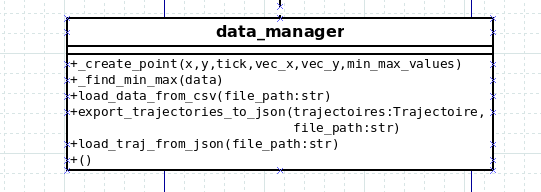
\includegraphics[scale=0.40]{img/utils.png}
                \caption{Diagramme UML du paquetage utils}
                \label{Diagramme_utils}
            \end{figure}
       \subsection{Paquetage model}
        La classe \texttt{Point} représente une position unique dans l'espace à un instant donné. Chaque point est défini par ses coordonnées $(x, y)$ ainsi qu’un marqueur temporel, appelé \texttt{tick}, qui permet d’ordonner les points dans la trajectoire d’un joueur. Cette classe fournit des méthodes d'accès aux coordonnées et au tick, facilitant ainsi l’exploitation des données par les autres composants du programme.\\
        
        À partir de ces points, la classe \texttt{Trajectoire} construit et manipule l’ensemble des déplacements d’un joueur. Lorsqu’une trajectoire est initialisée, elle associe un \texttt{player\_id} à une liste de points qui représentent les positions successives du joueur dans le temps.
        
        Un premier traitement effectué sur une trajectoire consiste à la découper en segments successifs. La méthode \texttt{sub\_trajectories} génère une liste de paires de points, chaque paire formant un segment de la trajectoire. Cette segmentation est essentielle pour l’analyse des mouvements puisqu’elle permet de comparer directement les déplacements élémentaires effectués entre deux instants consécutifs.  
        
        Pour des besoins d’analyse plus ciblés, la méthode \texttt{get\_partial\_segments} permet d’extraire un sous-ensemble de segments en fonction d’indices de départ et de fin. Ce filtrage permet, par exemple, de ne traiter qu’une portion de la trajectoire correspondant à une phase de jeu spécifique. Une validation des indices est effectuée pour éviter les erreurs liées aux dépassements de limites.  
        
        Au-delà des segments bruts, la méthode \texttt{get\_segments} enrichit la représentation en associant à chaque segment un vecteur déplacement et sa longueur. Grâce à la bibliothèque NumPy, le vecteur reliant deux points successifs est calculé, et sa norme est déterminée pour mesurer précisément la distance parcourue. 
        
        L’enchaînement des opérations dans le paquetage \texttt{model} suit ainsi une logique précise : les données brutes sous forme de points sont transformées en trajectoires, puis analysées sous forme de segments, avant d’être exploitées pour extraire des caractéristiques pertinentes sur les déplacements des joueurs. Ce processus permet d’organiser efficacement les trajectoires.
        
        \begin{figure}[H]
                \centering
                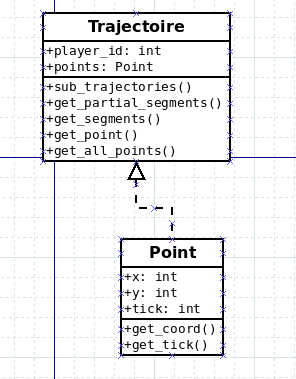
\includegraphics[scale=0.40]{img/model.png}
                \caption{Diagramme UML du paquetage Model}
                \label{Diagramme_model}
        \end{figure}

        \subsection{Paquetage algorithms}    

        Le paquetage \texttt{algorithms} contient des implémentations d'algorithmes visant à analyser et traiter les trajectoires des joueurs dans le contexte de l'analyse de données spatiales et temporelles. Ce paquetage regroupe plusieurs classes qui se concentrent sur des techniques de clustering, de partitionnement et de détection de motifs fréquents, afin de mieux comprendre les déplacements et comportements des joueurs au cours d'une partie.
    
        La classe \texttt{KMeans} implémente l'algorithme de clustering K-Means adapté aux données de trajectoires, prenant en compte la dimension temporelle des déplacements. Elle permet de regrouper les points d'une trajectoire en \texttt{k} clusters en utilisant une distance pondérée qui combine les distances spatiales et temporelles. La méthode \texttt{fit} effectue l'initialisation des centroids, l'attribution des points aux clusters et la mise à jour des centroids à chaque itération. La classe offre également une méthode \texttt{predict} pour attribuer de nouveaux points à leurs clusters respectifs, ainsi qu'une méthode \texttt{prepare\_data\_for\_prefixspan} pour préparer les données de clusters en vue d'une analyse par l'algorithme PrefixSpan.
    
        La classe \texttt{MDL} implémente l'algorithme MDL (Minimum Description Length) pour partitionner une trajectoire en segments significatifs. L'idée est de découper la trajectoire en segments qui minimisent la longueur de la description du modèle, en équilibrant la complexité de la partition et la précision de l'ajustement. La méthode \texttt{traj\_partitionning} divise une trajectoire en sous-ensembles en fonction de la minimisation du coût MDL, qui prend en compte des distances perpendiculaires et angulaires entre les segments successifs. Ce découpage permet d'identifier des phases distinctes dans les trajectoires des joueurs. Les calculs des distances sont réalisés par les méthodes privées \texttt{\_perpendicular\_distance} et \texttt{\_angular\_distance}, qui évaluent respectivement les distances géométriques et les similarités angulaires entre les segments de la trajectoire.
    
        La classe \texttt{PrefixSpanAnalyser} utilise l'algorithme PrefixSpan pour détecter les motifs fréquents dans les séquences de points de trajectoires. Elle prend en entrée un pourcentage de support minimal, qui détermine la fréquence d'apparition d'un motif pour qu'il soit considéré comme fréquent.\\
        La méthode \texttt{detectionFrequentPattern} applique l'algorithme PrefixSpan sur les séquences et retourne les motifs fréquents détectés. Cette classe permet ainsi d'extraire des motifs récurrents dans les déplacements des joueurs, fournissant des insights sur les comportements ou stratégies typiques au cours du jeu.
    
        Le paquetage \texttt{algorithms} permet d'exécuter ces algorithmes de manière efficace pour analyser les trajectoires des joueurs dans un environnement de jeu. Les techniques de clustering, de partitionnement MDL et de détection de motifs fréquents permettent de mieux comprendre et modéliser les dynamiques de jeu à partir des données spatiales et temporelles, facilitant ainsi l'analyse des stratégies et comportements des joueurs.

            \begin{figure}[H]
                \centering
                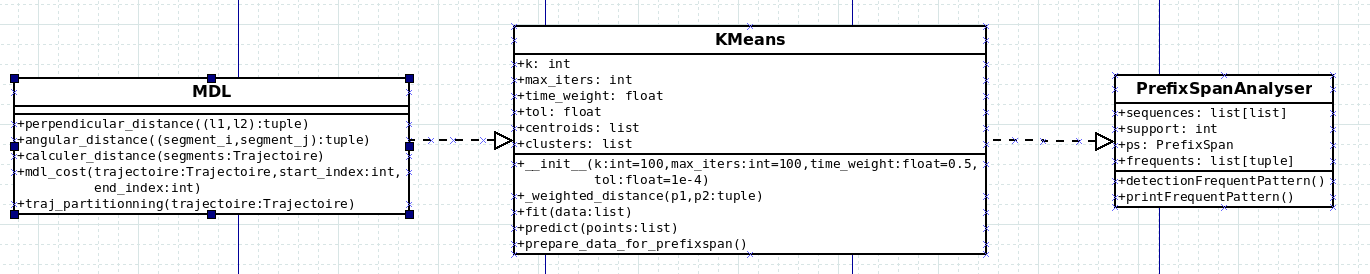
\includegraphics[width=\textwidth]{img/algorithms.png}
                \caption{Diagramme UML du paquetage Algorithms}
                \label{Diagramme_algorithms}
            \end{figure}

    \section{Structure globale}

        La chaîne de traitement dans vos différents exécutables suit une séquence logique d'étapes allant de l'importation des données brutes à leur transformation et nettoyage, jusqu'à leur analyse et leur exportation sous forme de résultats. Cette chaîne est structurée de manière à maximiser l'efficacité du traitement tout en facilitant la gestion et l'évolution du projet. Voici une explication détaillée de chaque étape de cette chaîne de traitement.
        
        \subsection{Importation des données (mainDataImport.py)}
        
        Le processus débute par l'importation des données. Ce fichier est responsable de la gestion des données brutes, généralement au format CSV, et de leur transformation en un format JSON structuré pour les étapes suivantes. Voici les principales étapes :
        
        \begin{itemize}
            \item \textbf{Vérification des fichiers existants :} Le script vérifie si des fichiers JSON sont déjà présents dans le répertoire \texttt{processed}. Si des fichiers JSON existent, ils sont chargés directement, et les trajectoires contenues dans ces fichiers sont traitées.
            \item \textbf{Chargement des fichiers CSV :} Si aucun fichier JSON n'est trouvé, le script cherche les fichiers CSV dans le répertoire \texttt{raw}. Les données CSV sont chargées, transformées en objets de type \texttt{Trajectoire}, puis exportées sous forme de fichiers JSON dans le répertoire \texttt{processed}.
        \end{itemize}
        
        Ainsi, cette étape se charge de préparer les données pour les étapes suivantes du pipeline.
        
        \subsection{Application de l'algorithme MDL (mainMDL.py)}
        
        Une fois les données JSON préparées, l'étape suivante consiste à appliquer l'algorithme MDL (Minimum Description Length) pour la partition des trajectoires. Le but ici est d'analyser les trajectoires et de les segmenter en sous-trajectoires significatives, en fonction de critères d'efficacité de compression (MDL).
        
        \begin{itemize}
            \item \textbf{Chargement des trajectoires :} Le script charge les fichiers JSON précédemment générés (contenant des trajectoires traitées) et les analyse.
            \item \textbf{Partitionnement des trajectoires :} Pour chaque trajectoire, l'algorithme MDL est appliqué pour la partitionner en sous-trajectoires. Cette étape génère une représentation plus concise de chaque trajectoire, facilitant une analyse plus détaillée des comportements observés.
            \item \textbf{Exportation des résultats :} Les résultats du partitionnement (les trajectoires segmentées) sont ensuite exportés sous forme de nouveaux fichiers JSON dans le répertoire \texttt{mdl}.
        \end{itemize}
        
        Cette étape se concentre donc sur la segmentation des données afin de les rendre prêtes pour des analyses plus poussées.
        
        \subsection{Application de l'algorithme KMeans (mainKMeans.py)}
        
        Une fois les trajectoires partitionnées, l'algorithme KMeans est appliqué pour regrouper les points de chaque trajectoire en clusters. Cela permet d'identifier des regroupements naturels dans les données, ce qui peut être utile pour comprendre les comportements des trajectoires.
        
        \begin{itemize}
            \item \textbf{Chargement des trajectoires MDL :} Le script charge les fichiers JSON contenant les trajectoires après l'application de MDL.
            \item \textbf{Application de KMeans :} Pour chaque trajectoire, les points sont extraits et utilisés pour entraîner un modèle KMeans, permettant de regrouper ces points en clusters.
            \item \textbf{Exportation des résultats :} Les résultats des regroupements (les nouvelles trajectoires après l'application de KMeans) sont exportés sous forme de nouveaux fichiers JSON dans le répertoire \texttt{kmeans}.
        \end{itemize}
        
        Cette étape permet de rendre les données plus interprétables en identifiant des groupes cohérents de points au sein des trajectoires.
        
        \subsection{Analyse des séquences fréquentes (mainPrefixSpan.py)}
        
        Une fois les trajectoires segmentées et regroupées, une dernière étape d'analyse est effectuée, consistant à identifier des motifs fréquents dans les trajectoires. L'algorithme PrefixSpan est utilisé à cet effet, afin de découvrir des séquences d'événements récurrentes.
        
        \begin{itemize}
            \item \textbf{Chargement des données KMeans :} Le script charge les fichiers JSON contenant les trajectoires après l'application de KMeans.
            \item \textbf{Analyse des motifs fréquents :} Les trajectoires sont analysées à l'aide de l'algorithme PrefixSpan, qui identifie les séquences d'événements les plus fréquentes au sein des données.
            \item \textbf{Affichage des résultats :} Les motifs fréquents identifiés sont affichés, et une représentation graphique des points moyens des trajectoires est générée pour aider à la visualisation des résultats.
        \end{itemize}

    \section{Expérimentation}
        \subsection{Format des données}

            Au départ, nous calculions les bornes de jeu dans une partie en fonction des données, sans prendre en compte les informations fournies (x borné par 66 et 188, et y borné par 72 et 186), ce qui a eu pour effet de compromettre nos données. Nous avons ensuite adapté en fonction de ces bornes, ce qui a permis de rendre la normalisation des données plus claire, précise, et commune à tous.

            Au départ, nous avons représenté les points uniquement avec les coordonnées. Puis, après réflexion, nous avons fait le choix d’y ajouter le tick pour une meilleure représentation temporelle.

            Les données fournies étaient au format CSV. Nous avons choisi de tout transformer et de stocker dans des fichiers JSON pour plusieurs raisons :
            \begin{itemize}
            \item Temps d'import, d'export.
            \item Poids des fichiers.
            \item Clarté lors d'une lecture simple et rapide.
            \end{itemize}
            Voici un exemple de structure JSON pour les données normalisées et après le passage de MDL (pour K-Means, le tick d'un centroid sera uniquement son index dans la liste de retour) :
            \newpage
            \begin{lstlisting}[language=json]
            {
            "PlayerId": 1,
            "points": [
            {
            "x": 116.65819512038934,
            "y": 177.87679002192982,
            "tick": 28320.0
            },
            {
            "x": 106.00205718493852,
            "y": 247.30481599506578,
            "tick": 28410.0
            },
            {
            "x": 103.57265785092214,
            "y": 287.56017852247805,
            "tick": 2
            }
            ]
            }
            \end{lstlisting}
        \subsection{Poids du temps dans K-Means}
        Comme expliqué précédemment, nous avons mis en place une pondération temporelle dans le calcul des distances entre les centroids. Nous avons mené quelques expérimentations à ce sujet, et nous avons choisi de mettre en place une pondération à 50/50 entre le temps et la position, ce qui permet d’obtenir des résultats homogènes, lisibles et adaptés à Prefix-Span.
        
        \subsection{Prefix-Span et support}

            Lors des premières utilisations de PrefixSpan, nous ne trouvions soit aucun résultat à cause d'un support trop élevé, soit nous trouvions des résultats totalement incohérents, de type :
            \begin{itemize}
            \item Des patterns "immobiles".
            \item Des patterns de morts, c’est-à-dire que le joueur retourne au niveau de son lieu d’apparition.
            \item Des patterns illisibles avec un ou plusieurs points hors de l’aire de jeu.
            \item Des patterns "au milieu", tout simplement.
            \end{itemize}
            Pour résoudre ces problèmes, nous avons trouvé quatre solutions que nous allons détailler ci-dessous.

            Prefix-Span étant un algorithme de détection de patterns fréquents avec des motifs "identiques" et les centroids résultant de K-Means étant des moyennes, la probabilité qu’ils soient identiques entre les parties est quasi nulle. Il était donc impossible de trouver des patterns en utilisant Prefix-Span. Nous avons donc choisi d’effectuer un arrondi en fonction d’un quadrillage de l’aire de jeu 10x10, ce qui rend possible la détection de patterns grâce à Prefix-Span.

            Le support fait partie intégrante de Prefix-Span, il représente le pourcentage de trajectoires dans lesquelles nous retrouvons un pattern. Nous avons testé différents supports afin de comparer le nombre de résultats.
            Voici les résultats :
             \begin{center}
                    \begin{tabular}{|c|c|}
                        \hline
                        Support & Nombre de patterns \\
                        \hline
                        5 & 400 000 \\
                        \hline
                        10 & 26 500 \\
                        \hline
                        15 & \textcolor{red}{215} \\
                        \hline
                        17.5 & 1 \\
                        \hline
                        20 & 0 \\
                        \hline
                        25 & 0 \\
                        \hline
                    \end{tabular}
                \end{center}
            Nous avons conclu de ces expérimentations que le fait de trouver environ 215 patterns est le plus pertinent à analyser. Nous avons donc opté pour un support de 15 pour la suite de nos expérimentations.
            

            Après avoir déterminé le support idéal pour une bonne analyse complète, nous avons remarqué que de nombreux patterns étaient pollués par des coordonnées "fantômes" hors de la carte de jeu, ce qui faussait totalement notre normalisation des données. Nous avons donc choisi de supprimer ces coordonnées des trajectoires.
            Ensuite, nous avons constaté que certaines trajectoires étaient totalement vides, c’est-à-dire que soit le joueur ne bougeait pas de son lieu d’apparition en début de partie, soit il restait hors de la carte de jeu durant toute la durée de la partie. Nous avons donc décidé de supprimer complètement ces trajectoires lors de la normalisation des données.
            

            Après avoir corrigé la normalisation des données et déterminé le support idéal pour Prefix-Span, nous avons remarqué que la plupart des patterns se regroupaient au milieu de la carte de jeu. Nous en avons conclu que le fait de regrouper les coordonnées des joueurs de chaque équipe (avec des coordonnées "symétriques") empêchait l’identification de patterns autres qu’une simple présence commune au centre de l’aire de jeu.
            

            Après nous être renseignés sur le déroulement d’une partie de DOTA2, nous nous sommes rendus compte que nous pouvions la partitionner en trois phases distinctes :
            \begin{enumerate}
            \item 0-20 min -> Early Game, phase de préparation sur sa voie (en fonction de son poste).
            \item 20-40 min -> Mid Game, combats pour les objectifs et en équipe.
            \item 40 min - fin de partie -> End Game, combats et prise d’objectifs décisifs pour le résultat final.
            \end{enumerate}
            Nous avons donc décidé de refaire tourner chacun de nos algorithmes sur des données partitionnées en fonction de ces phases de jeu afin de détecter des patterns propres à chacune d’elles.
            
        \subsection{Format de visualisation des résultats}
        Afin de visualiser les différents patterns et de détecter différentes stratégies, nous avons fait le choix de superposer une image de la carte de jeu sur nos graphiques. Cela nous permet de détecter des points de passage importants pour le déroulement d’une partie.

        \begin{figure}[htbp]
            \centering
            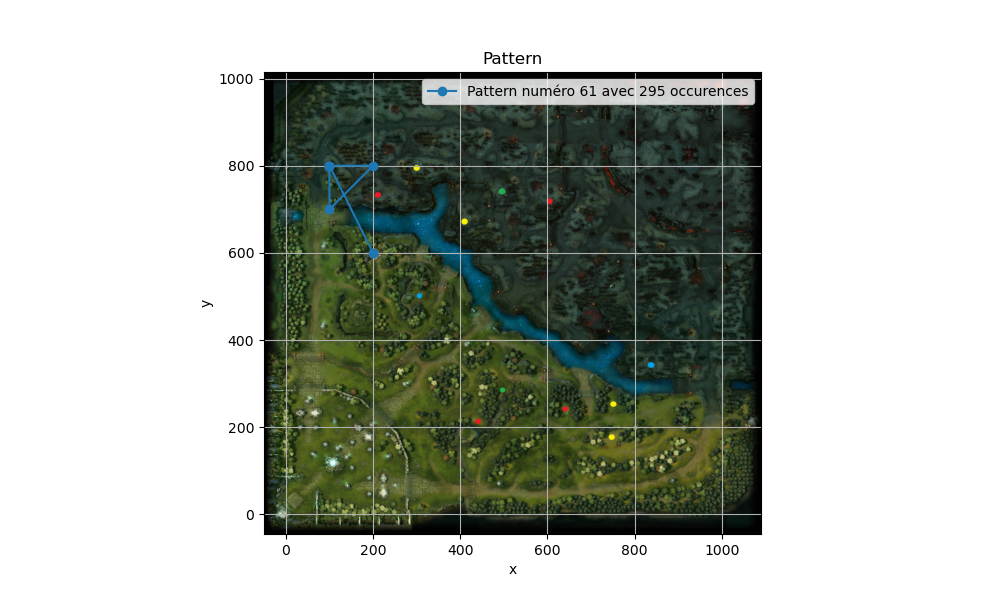
\includegraphics[scale=0.5]{img/prefixEarly.png}
            \caption{Exemple d'un affichage de pattern}
            \label{test_mdl}
        \end{figure}
    

    \section{Conclusion et améliorations possibles}
        \subsection{Résultats obtenus}
        Après toutes ces expérimentations nous obtenons des résultats satisfaisant. En effet nous arrivons, en découpant notre partie en 3 phases, a identifier des schémas de jeu pour chacune d'entre-elles.

        \begin{itemize}
            \item Early Game : Les joueurs sont à leurs postes sur leur voies. On le repère par les patterns correspondant à des coordonnées de voies (100, 800) pour la voie du haut, (400,500) pour la voie du milieu ou (800, 100) pour celle du bas. Des patterns de déplacement entre des positions sur une même voie montrent que les joueurs tiennent leurs postes durant cette phase de jeu. On a donc une stratégie commune pour les deux équipes pour la quasi-totalité des parties.

            \item Mid Game : Cette phase est plus compliquée a analyser. Malgré des réglages de support, des arrondis et autres expérimentations, nous n'arrivons pas à retrouver de stratégie. On suppose que cela est dû à une diversification des schémas en fonction des personnages joués ou encore des équipes. Nous ne repérons pas de patterns mais peut-être qu'un fichier de données plus complet ou encore l'implémentation d'autres algorithmes de détection que le Prefix-Span nous l'aurait permis.

            \item End Game : Les patterns communs a cette phase sont les stratégies de défense, lorsqu'une équipe est acculée dans sa base. On suppose donc que les stratégies d'attaque varient selon les parties mais qu'une équipe défendra toujours plus ou moins de la même façon. On distingue également plus de schémas défensives chez l'équipe en bas à gauche. Cela laisse à supposer que dans Dota2, au moment où on était enregistré ces parties, il y a un avantage pour l'équipe du haut.
        \end{itemize}

        \subsection{Axes d'amélioration}
        Pour notre projet, si nous avions eu plus de temps, nous pourrions implémenter un autre algorithme de clustering, par exemple l'algorithme de propagation d'affinité. Avec ces résultats, nous aurions pu faire des comparaisons avec les résultats actuels et éventuellement avoir de nouvelles informations sur les stratégies des joueurs.
        De plus, nous avons utilisé un package prefixspan déjà programmé, nous pourrions très bien programmer notre propre algorithme qui ne sert que nos intérêts précis. Cela pourrait parfaire nos résultats.\\
        Avec d'autres données et d'autres informations, comme notamment le rôle de chaque joueur dans la partie, nous pourrions améliorer l'accès à certaines stratégies en ciblant seulement certains postes et en discriminant d'autres rôles.
        
        


\end{document}
